\documentclass{beamer}
%\documentclass{beamer}
\usetheme{JuanLesPins}
\usepackage{epsfig, graphics, graphicx,subfigure, amsmath, tabularx, verbatim}
\usepackage[spanish,es-tabla]{babel}
\decimalpoint
\usepackage{gensymb}
\usepackage[utf8]{inputenc}
\usepackage[T1]{fontenc}
\makeatletter
\newcommand\titlegraphicii[1]{\def\inserttitlegraphicii{#1}}
\titlegraphicii{}
\setbeamertemplate{title page}
{
	\vbox{}
	{\usebeamercolor[fg]{titlegraphic}\inserttitlegraphic\hfill\inserttitlegraphicii\par}
	\begin{centering}
		\begin{beamercolorbox}[sep=8pt,center]{institute}
			\usebeamerfont{institute}\insertinstitute
		\end{beamercolorbox}
		\begin{beamercolorbox}[sep=8pt,center]{title}
			\usebeamerfont{title}\inserttitle\par%
			\ifx\insertsubtitle\@empty%
			\else%
			\vskip0.25em%
			{\usebeamerfont{subtitle}\usebeamercolor[fg]{subtitle}\insertsubtitle\par}
			\fi%     
		\end{beamercolorbox}%
		\vskip1em\par
		\begin{beamercolorbox}[sep=8pt,center]{author}
			\usebeamerfont{author}\insertauthor
		\end{beamercolorbox}
		\begin{beamercolorbox}[sep=8pt,center]{date}
			\usebeamerfont{date}\insertdate
		\end{beamercolorbox}
		
	\end{centering}
	\vfill
}

%
\titlegraphic{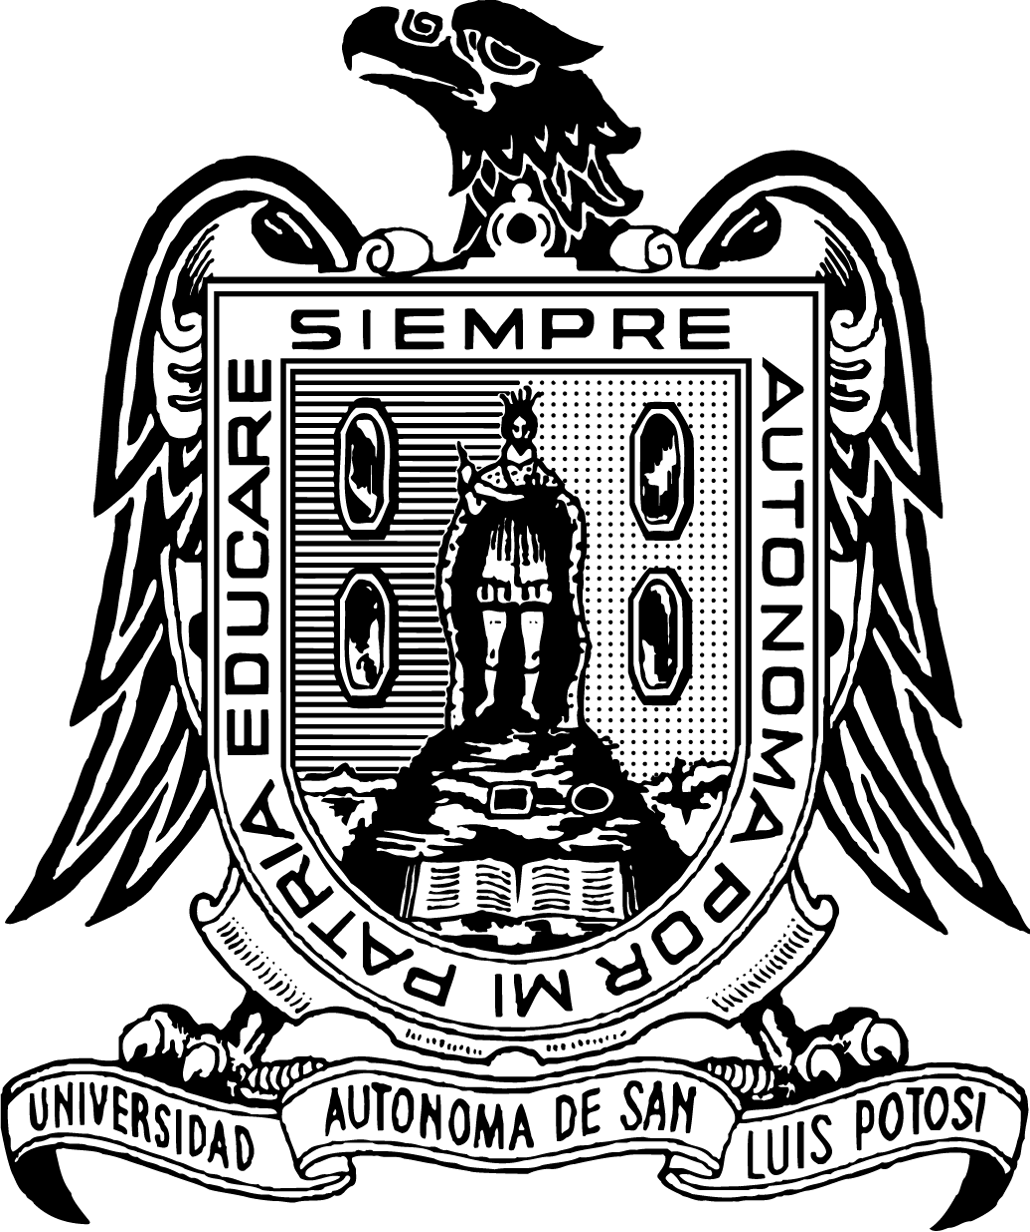
\includegraphics[scale=0.2]{portada/escudouaslp.png}}
\titlegraphicii{
\includegraphics[scale=0.15]{portada/escudofciencias.png}}
\title{Estudio te\'orico de propiedades magn\'eticas en [Pt,V] (Se,S)\textsubscript{2} y experimentación de efecto Kerr en CoFeB}
\subtitle{Examen de defensa de tesis}
\author{Gabriel Adona\'i Mart\'inez Zepeda\\ \textbf{Asesor:} Dr. Ra\'ul Balderas Navarro}
\institute{Universidad Aut\'onoma de San Luis Potos\'i\\ Facultad de Ciencias}
\date{\today}


%

\usepackage[backend=bibtex,style=numeric, defernumbers=true]{biblatex}
\bibliography{ref,refInt,refKerr,refMet,refSim,refRel}
\setbeamertemplate{bibliography item}{}
\includeonly{
	intrPress,
	dftPress,
	metodosComp,
    resultadosSim1,
	kerr, 
    montaje, 
	analisis, 
	mediciones,
	concl
}
\setbeamertemplate{footline}[frame number]
\setbeamertemplate{caption}[numbered]
\begin{document}
	\frame[plain]{\titlepage}
	\frame[allowframebreaks]{\frametitle{Contenidos} \tableofcontents}
	\section{Introducci\'on}
\frame{
	\frametitle{Introducci\'on}
	
	\begin{itemize}
		\item Los procesos físicos basados en el spin representan una parte fundamental en el estudio de la materia condensada y, aunque existen todav\'ia algunas cuestiones que no han sido explicadas satisfactoriamente, como el acople spin-\'orbita, la interacci\'on fot\'on-spin, el ordenamiento de spines en bajas dimensiones.
		\item Se busca el estudio de propiedades magn\'eticas en materiales bidimensionales, adem\'as de estudiar la variaci\'on de \'esta si se le aplica una deformaci\'on mec\'anica.
		\item se implement\'o un sistema de espectroscop\'ia Kerr para el estudio de materiales magn\'eticos.  
	\end{itemize}
}
	\section{Estudio te\'orico de materiales Bidimensionales}
\subsection{Teor\'ia Funcional de la densidad}
\frame{
	\begin{figure}[!hbt]
		\centering
		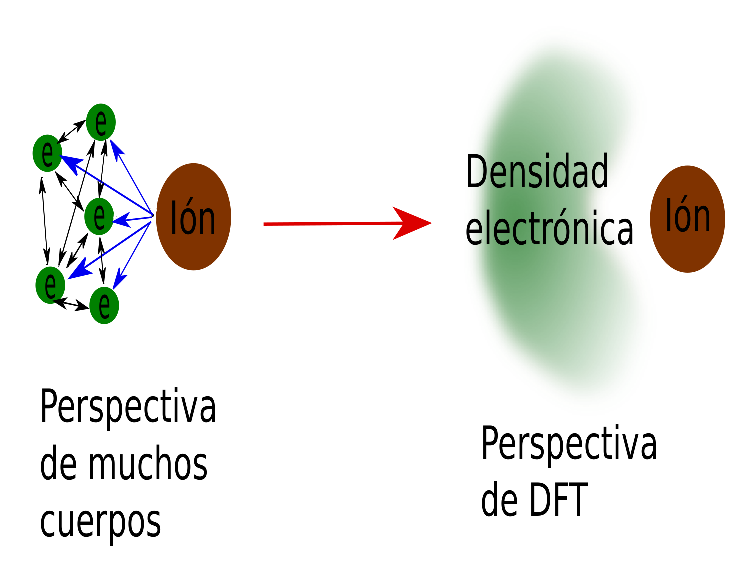
\includegraphics[width=7.0cm,height=7.0cm]{figuras/perspectivaDFT.eps}
		\caption[Perspectiva de la teor\'ia Funcional de la Densidad.]{Idea de la Teor\'ia Funcional de la Densidad.}
		\label{im:dftIdea}
	\end{figure}
}
\frame{
	\frametitle{Ecuaci\'on de Schrödinger de muchos cuerpos}
	La ecuaci\'on fundamental para c\'alculos \textit{ab initio} es la de Schr\"odinger cuyo Hamiltoniano es:
	\begin{multline}
		\hat H = - \frac{\hbar ^2}{2 m_e} \sum_{i} \nabla_{i}^2 - \sum_{i,I} \frac{Z_I e^2}{\vert \pmb{r_i} - \pmb{R_I} \vert}+ \frac{1}{2} \sum_{i \not= j}  \frac{e^2}{|\pmb{r_i} - \pmb{r_j} |}\\
		- \sum_{I} \frac{\hbar^2}{2 M_I} \nabla_I^2 + \frac{1}{2} \sum_{I \not= J} \frac{Z_I Z_J e^2}{|\pmb{R_I}-\pmb{R_J}|}  \label{ec:sh} 
	\end{multline}	
}

\frame{
	\begin{equation}
		\hat H = \hat T + \hat V_{ext} + \hat V_{int}+E_{II} \label{ec:shelectron}
	\end{equation}
    \pause
    \vspace{0.3cm}
    \begin{equation}
    	\hat{T} = \sum_{i} -\frac{1}{2} \nabla_{i}^2 ,\label{ec:shT}
    \end{equation}
    \pause
    \vspace{0.3cm}
    	\begin{equation}
    	\hat{V}_{ext} = \sum_{i,I} V_I (|\pmb{r_i}-\pmb{R_I}|), \label{ec:shVex}
    \end{equation}
    \pause
    \vspace{0.3cm}
    	\begin{equation}
    	\hat{V}_{int} = \frac{1}{2} \sum_{i \not= j} \frac{1}{|\pmb{r_i}-\pmb{r_j}|} \label{ec:shVint}
    \end{equation}
}
\frame{
	\frametitle{Definiciones de la densidad y magnetizaci\'on}
	\begin{itemize}
		\item Densidad de electrones:
		\begin{equation}
			n_{s ', s }(\pmb{r})= \delta_{s',s} \sum_{i} \psi_{i,s '}^ {*} (\pmb{r}) n_{i,s}~ \psi_{i,s } (\pmb{r}). \label{ec:denspin}
		\end{equation}
	   \pause
	   \item Magnetizaci\'on:
	   \begin{equation}
	   	\pmb{m} (\pmb{r}) = - \mu_{B} \sum_{s,s '} \pmb{\sigma}_{s,s'}~ n_{s ', s }(\pmb{r}) , \label{ec:magn}
	   \end{equation}
	\end{itemize}
}
\begin{comment}


\frame{
	\frametitle{Componentes de la magnetizaci\'on}
	\begin{subequations} \label{ec:compm}
		\begin{gather}
			m_x (\pmb{r})= -2 ~\mu_{B} ~Re~ n_{\uparrow, \downarrow} (\pmb{r}) \label{ec:compm1}\\
			m_y (\pmb{r})= -2 ~\mu_{B} ~Im~ n_{\uparrow, \downarrow} (\pmb{r}) \label{ec:compm2}\\
			m_z (\pmb{r}) = - \mu_{B} ~[n_{\uparrow, \uparrow} (\pmb{r})- n_{\downarrow, \downarrow} (\pmb{r})] . \label{ec:compm3}
		\end{gather}
	\end{subequations}
}
\end{comment}
\subsubsection{Teoremas de Hohenberg-Kohn}
\frame{
	\frametitle{Primer teorema de Hohenberg-Kohn}
	\begin{figure}[!hbt]
		\centering
		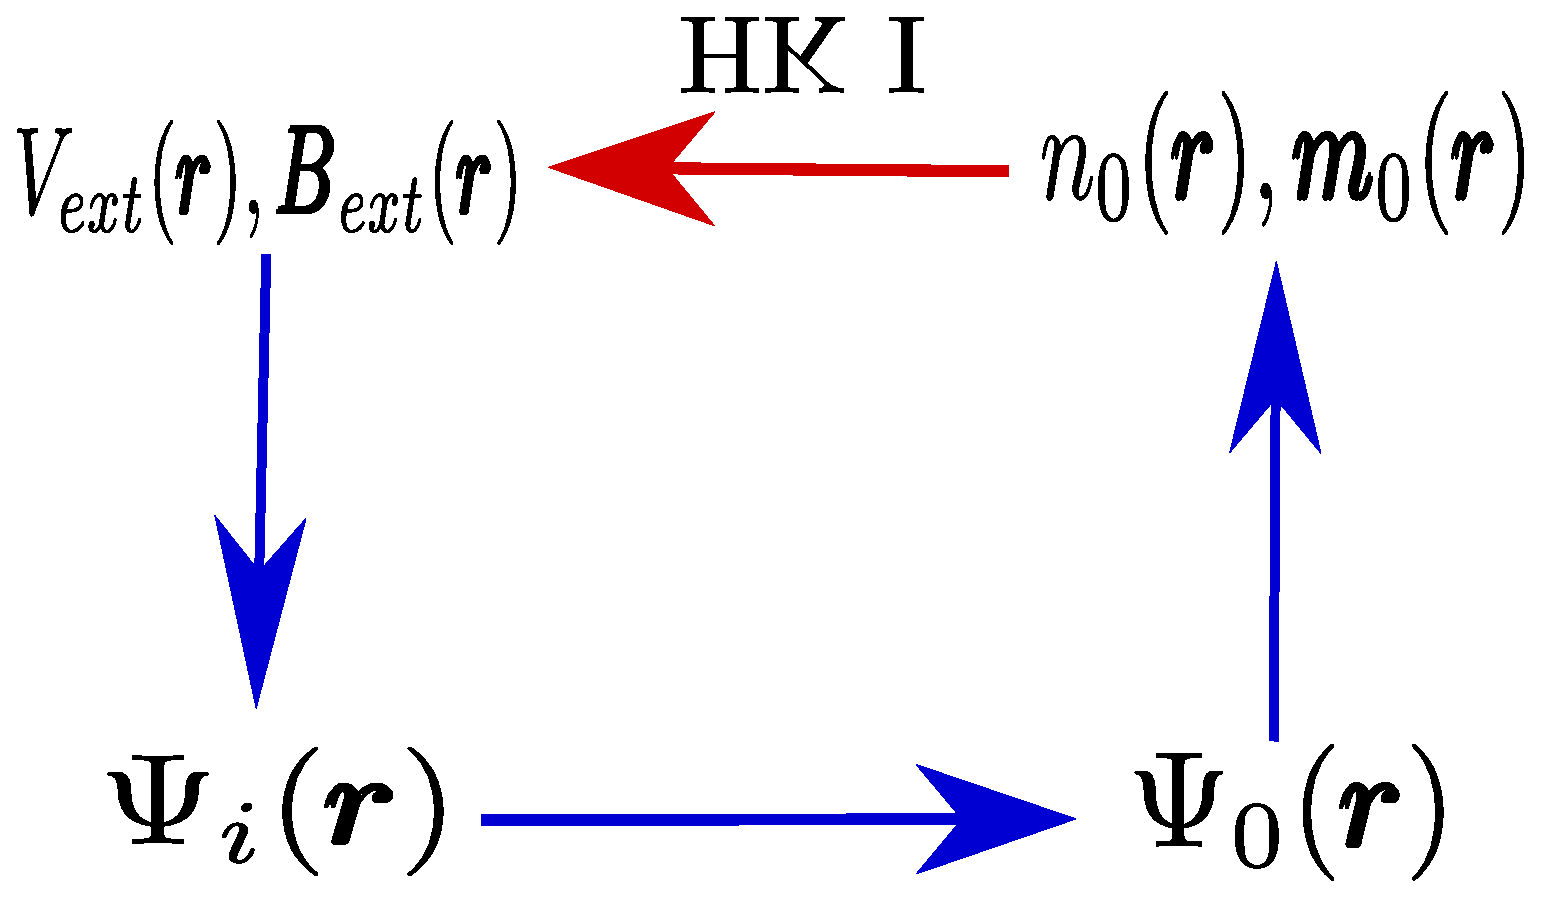
\epsfig{file=figuras/HK1.eps, width=6.0cm,height=5.0cm}
		\caption[Primer teorema de Hohenberg-Kohn]{Representaci\'on esquem\'atica del primer teorema de Hohenberg-Kohn}
		\label{fig:hk1}
	\end{figure}
}
\frame{
  \frametitle{Segundo teorema de Hohenberg-Kohn}
  \begin{equation}
  	E_0 = \min_{n  \to n_0, \pmb{m} \to \pmb{m}_0} E_{V_{ext}, \pmb{B}_{ext}}[n,\pmb{m}]  \label{ec:HKII}.
  \end{equation}
  \pause
  \vspace{0.7cm}
  \begin{equation}
  	E_{V_{ext}, \pmb{B}_{ext}}[n,\pmb{m}]= F[n,\pmb{m}] + \int d \pmb{r} \{V_{ext} (\pmb{r}) n(\pmb{r})+\pmb{B}_{ext} (\pmb{r}) \cdot \pmb{m} (\pmb{r}) \} +E_{II}, \label{ec:funcional}
  \end{equation}
\pause
 \begin{eqnarray}
	F[n,\pmb{m}]&= \langle \Psi_0 [n,\pmb{m}]| \hat{T}+\hat{V}_{int} | \Psi_0 [n,\pmb{m}] \rangle \nonumber \\
	&= T[n,\pmb{m}] + V_{int} [n,\pmb{m}]. \label{ec:funcF}
\end{eqnarray}
}
\subsubsection{Ecuaciones de Kohn-Sham}
\frame{
	\frametitle{Ecuaciones de Kohn-Sham}
	\begin{equation}
		(H_{KS}^s -\epsilon_{i,s})~\psi_{i,s } (\pmb{r}) = 0 \label{ec:ShKS},
	\end{equation}
    \pause
      \vspace{0.3cm}
    \begin{equation}
    	H_{KS}^s = -\frac{1}{2} \nabla^2 + V_{KS}^s (\pmb{r}), \label{ec:HamiltonianoKS}
    \end{equation}
	\pause
	\vspace{0.3cm}
	 \begin{eqnarray}
		V_{KS}^s (\pmb{r}) &=& V_{ext} (\pmb{r})+  \frac{\delta E_{Hartree}}{\delta n_s (\pmb{r})}+  \frac{\delta E_{XC}^s}{\delta n_s (\pmb{r})} \nonumber \\
		&=& V_{ext} (\pmb{r})+ V_{Hartree} (\pmb{r}) + V_{XC}^s (\pmb{r}). \label{ec:potKS} 
	\end{eqnarray}
}
\frame{
	\begin{equation}
		E_{Hartree} = \int d \pmb{r} d \pmb{r'} \frac{n(\pmb{r}) n(\pmb{r'})}{|\pmb{r}-\pmb{r'}|} \label{ec:Hartree}.
	\end{equation}
    	\vspace{0.3cm}
    \begin{equation}
    	E_{XC}^s [n]= \langle \hat{T} \rangle - T_{sp} [n]+\langle \hat{V}_{int} \rangle-E_{Hartree} [n] \label{ec:Exc2},
    \end{equation}
}
\begin{comment}


\subsubsection{Aproximaci\'on PBE}
\frame{
	\frametitle{Aproximaci\'on de gradientes generalizados}
	\begin{multline}
		E_{XC}^{GGA} [n_{\uparrow} (\pmb{r}), n_{\downarrow}(\pmb{r})] = \\ \int d^3 r ~ n(\pmb{r}) \epsilon_{XC} \left(n_{\uparrow} (\pmb{r}), n_{\downarrow}(\pmb{r}), \left|\nabla n_{\uparrow} (\pmb{r}) \right|^2, \left|\nabla n_{\downarrow} (\pmb{r}) \right|^2 \right)  \\
		= \int d^3 r ~ n(\pmb{r}) \epsilon_{X}^{hom} (n) F_{XC} \left(n_{\uparrow} (\pmb{r}), n_{\downarrow}(\pmb{r}), \left|\nabla n_{\uparrow} (\pmb{r}) \right|^2, \left|\nabla n_{\downarrow} (\pmb{r}) \right|^2 \right), \label{ec:funcXCGGA}
	\end{multline}
  \pause
  $ \epsilon_{X}^{hom} (n) = -3k_F / 4\pi $
}
\end{comment}
\frame{
	\frametitle{Ecuaciones de kohn-Sham para el caso no colineal}
	\begin{multline}
		\sum_{s}  \left[-\frac{1}{2} \nabla^2 + V_{ext} (\pmb{r})+ V_{Hartree} (\pmb{r}) + V_{XC} (\pmb{r}) \right] \delta_{s',s}  \phi_{\Lambda} (\pmb{r},s)\\ - \mu_{B} \sum_{s}  [\pmb{B}_{ext} (\pmb{r})+ \pmb{B}_{XC} (\pmb{r}) ] \pmb{\sigma_{s,s'}} \phi_{\Lambda} (\pmb{r},s) = \varepsilon_{\Lambda} \phi_{\Lambda} (\pmb{r},s) , \label{ec:KSnoColl}
	\end{multline}
\pause
 \begin{equation*}
	B_{XCj} (\pmb{r}) = - \frac{\delta E_{XC} [n,\pmb{m}]}{\delta m_j (\pmb{r})} \label{ec:Bxc},
\end{equation*}
}
	\subsection{M\'etodos computacionales}
\frame{
	\frametitle{M\'etodos computacionales}
	\begin{itemize}
		\item Se Utiliza el software Quantum-Espresso para realizar los c\'alculos de primeros principios.
		\pause
		\item Se utilizan dos computadoras que se encuentran equipadas con un procesador con 8 n\'ucleos y 32 GB de memoria RAM.
	\end{itemize}
}
\subsubsection{Materiales}
\frame{
	\frametitle{Materiales}
	\begin{columns}
		\column{0.4\textwidth}
		       \begin{figure}
		       	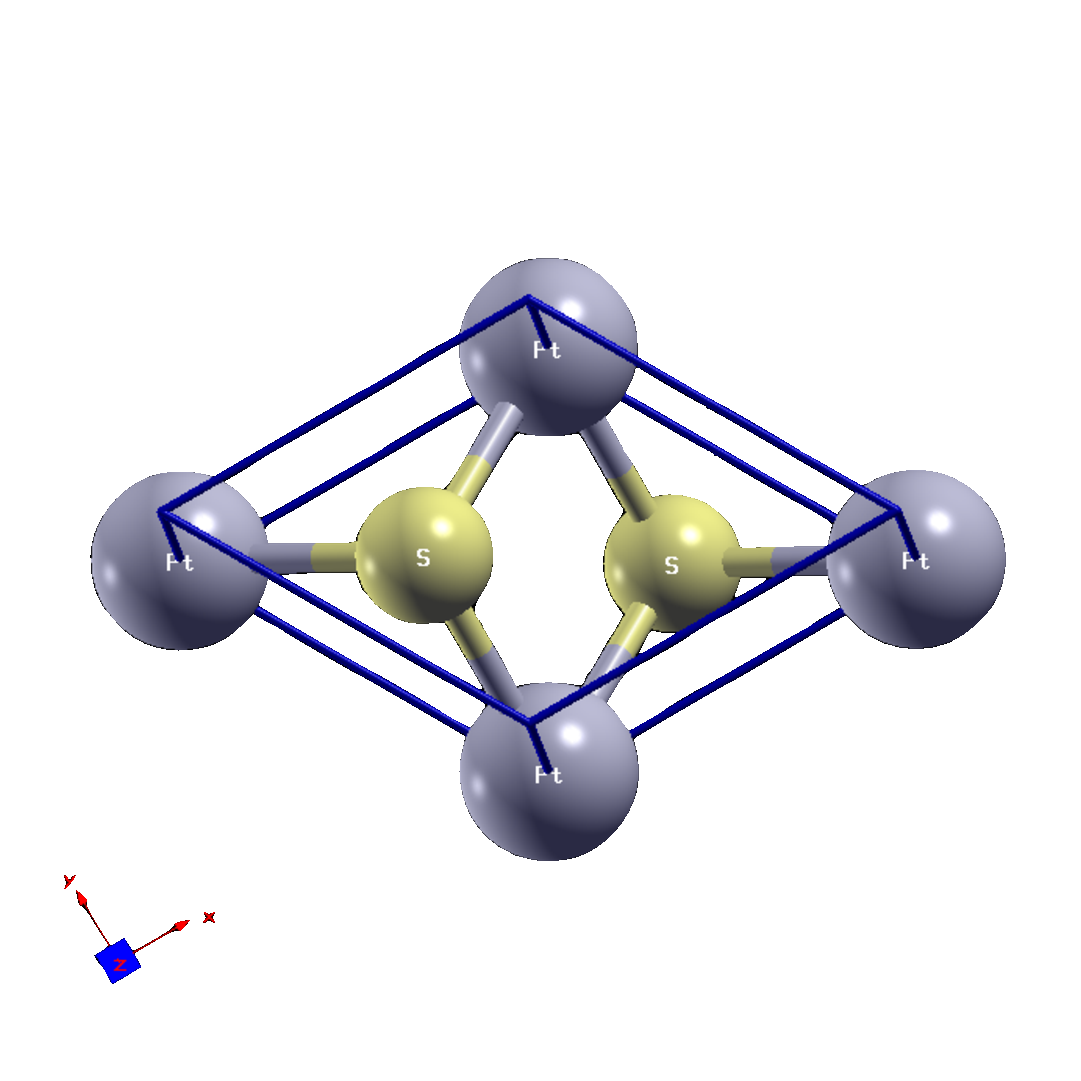
\epsfig{file=figMet/superceldaarriba.eps, width=5.0cm,height=5.0cm}
		       	\caption{Supercelda para c\'alculos sin defectos.}
		       \end{figure}
		    	
		%
		\column{0.6\textwidth}
		\begin{itemize}
			\item Estructura $1T$.
			\pause
			\item PtSe\textsubscript{2}, PtS\textsubscript{2}, VSe\textsubscript{2} y VS\textsubscript{2}
			\pause
			\item Modelos de materiales creados en VESTA a partir de estructuras disponibles en una base de datos en donde se le agrega una capa de vac\'io.
		\end{itemize}
	\end{columns}
}
\frame{
	\frametitle{Tabla peri\'odica}
	\begin{figure}[!hbt]
		\centering
		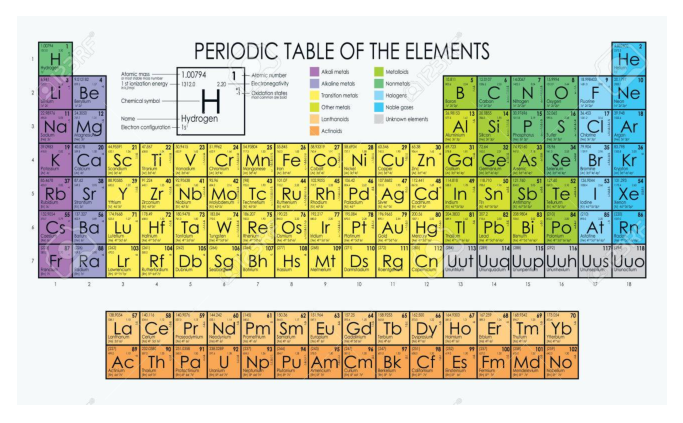
\epsfig{file=figRes/tabla-periodica-de-los-elementos.eps, scale=1}
	\end{figure}
	
}
\frame{
	\frametitle{Orbitales de los \'atomos utilizados}
	\begin{itemize}
		\item Metales de transici\'on:
		\pause
		\begin{itemize}
			\item Pt $\leftarrow~~5d^{9}~ 6s^{1}$
			\pause
			\item V $\leftarrow~~3d^{3}~4s^2$
		\end{itemize}
	    \pause
	    \item Calc\'ogenos:
	    \begin{itemize}
	    	\item S $\leftarrow~~3s^{2} ~3p^{4}$
	    	\pause
	    	\item Se $\leftarrow~~4s^{2} ~4p^{4}$
	    \end{itemize}
	\end{itemize}
}
\begin{frame}{Valores para la energ\'ia de corte y mapeo de Monkhorst y Pack}
	\begin{table}
		\caption[Valores de la energ\'ia de corte y mapeo de Monkhorst-Pack.]{Muestra los valores para la energ\'ia de corte y el mapeo en el espacio rec\'iproco (mapeo de Monkhorst y Pack) para las estructuras utilizadas en este trabajo.}
		\begin{tabular}{|c|c|m{5 cm}|} 
			\hline
			Material       &   $E_{corte}~~(Ry)$     & mapeo de Monkhorst y Pack $(k\times k \times 1)$  \\
			\hline
			\hline
			$PtS_2$        &   $60 $             &  $~~~~~~11 \times 11 \times 1$ \\
			$PtSe_2$        &   $63 $             &  $~~~~~~11 \times 11 \times 1$ \\
			$VS_2$        &   $80 $             &  $~~~~~~21 \times 21 \times 1$ \\
			$VSe_2$        &   $84 $             &  $~~~~~~21 \times 21 \times 1$ \\
			\hline
		\end{tabular}
	\end{table}
\end{frame}
\subsubsection{Creaci\'on del modelo de  la  vacancia de metal de transici\'on}
\frame{
	\frametitle{Creaci\'on del modelo de  la  vacancia de metal de transici\'on}
	\begin{columns}
		\column{0.4\textwidth}
		\begin{figure}
			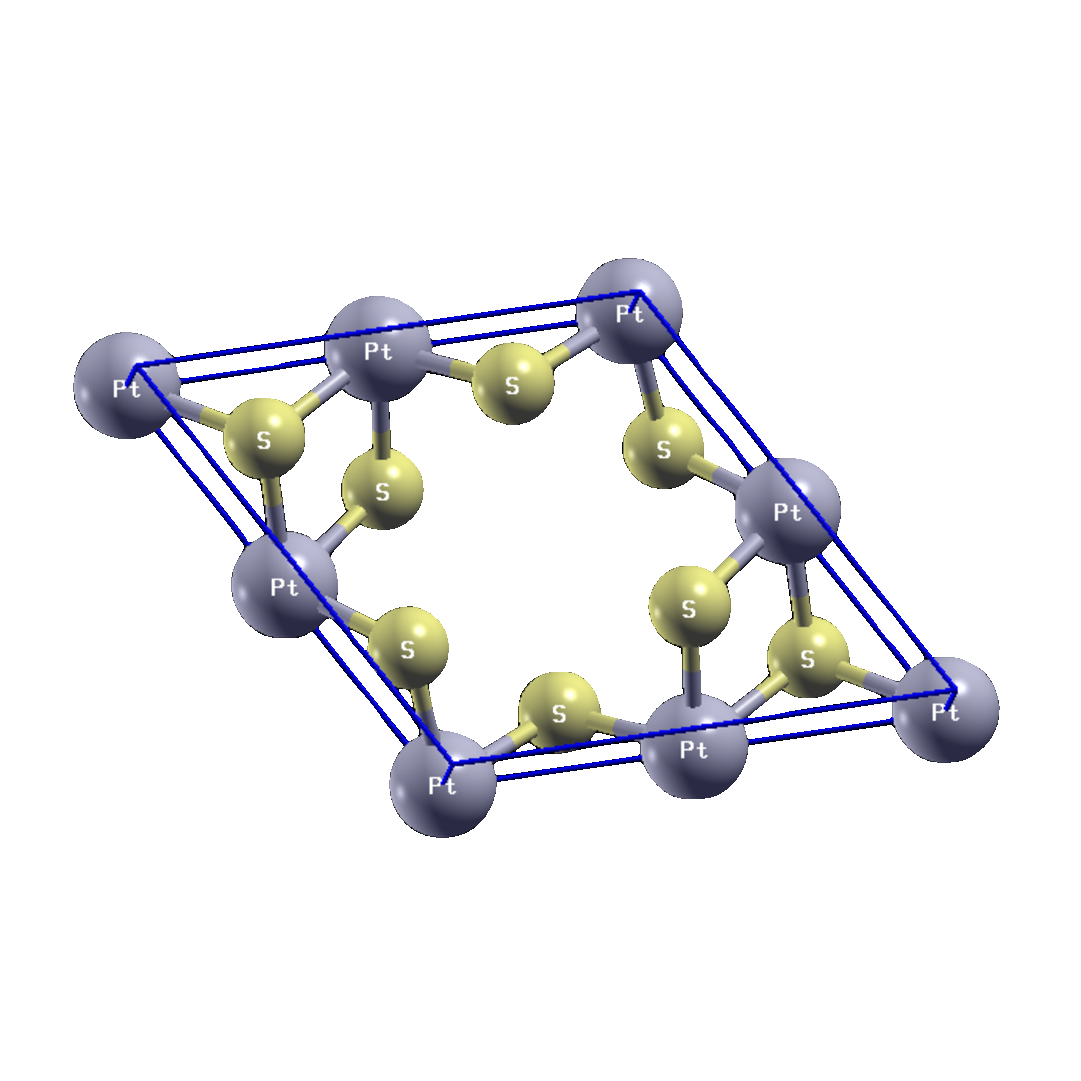
\epsfig{file=figMet/superceldaVacanciaArriba.eps, width=5.0cm,height=5.0cm}
			\caption{Supercelda para c\'alculos con vacancia del metal de transici\'on.}
		\end{figure}
			
		%
		\column{0.6\textwidth}
			\begin{itemize}
				\item Se crean con VESTA repitiendo dos veces la celda unitaria en las direcciones $a$ y $b$
				\pause
				\item Es necesario realizar una optimizaci\'on geom\'etrica.
			\end{itemize}
	\end{columns}
}	
\subsubsection{Deformaciones mec\'anicas}
\frame{
	\frametitle{Deformaciones mec\'anicas}
	\begin{figure}[hbt!]
		\centering
		\subfigure[]{
			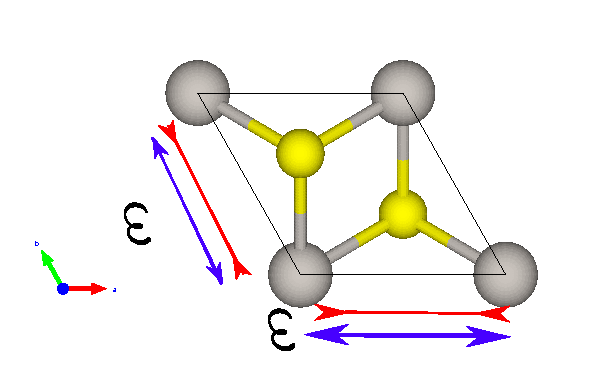
\epsfig{file=figMet/strainIso.eps, scale=0.5}
			\label{Met:fig:strainiso}
		}
		\subfigure[]{
			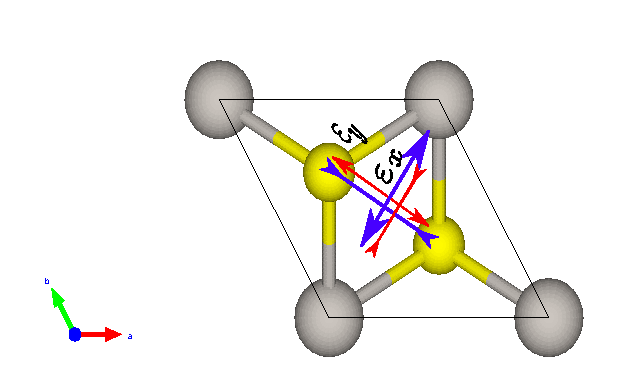
\epsfig{file=figMet/strainIAnis.eps, scale=0.5}
			\label{Met:fig:strainanis}
		}	
		\caption[Deformaciones estudiadas.]{Deformaciones estudiadas en este trabajo. \ref{Met:fig:strainiso} Muestra la aplicaci\'on de una deformaci\'on isotr\'opica en direcci\'on de los ejes cristalinos y \ref{Met:fig:strainanis} una deformaci\'on dirigida en la direcci\'on de los ejes cartesianos.}
	\end{figure}
}
\frame{
	\begin{itemize}
		\item Para el c\'alculo de la deformaci\'on se utiliza la siguiente expresi\'on:
		\begin{equation}
			\varepsilon = \frac{a-a_0}{a_0}. \label{Met:ec:strain}
		\end{equation}
	\pause
	\item Despu\'es de aplicar esta deformaci\'on es necesario realizar una optimizaci\'on geom\'etrica para que los \'atomos se coloquen en su nueva posici\'on de equilibrio.
	\end{itemize}
}
\begin{comment}


\subsubsection{C\'alculos realizados con Quantum Espresso}
\frame{
	\frametitle{C\'alculos realizados con Quantum Espresso}
	\begin{itemize}
		\item Evaluaci\'on auto consistente por medio del programa pw.x para encontrar la energ\'ia total del sistema, para realizar la optimizaci\'on geom\'etrica y el c\'alculo de la magnetizaci\'on.
		\pause
		\item Se utiliza pw.x para realizar un c\'alculo no auto consistente necesario para obtener el diagrama de bandas y la densidad de estados.
		\pause
		\item El programa band.x se usa para el c\'alculo del diagrama de bandas, dos.x para el c\'alculo de la densidad de estados y projdos.x para obtener la densidad de estados proyectada en los orbitales at\'omicos.
	\end{itemize}
}
\end{comment}
\frame{
	\frametitle{Par\'ametros de los c\'alculos auto consistentes}
	\begin{itemize}
		\item Se utiliza la aproximaci\'on de PBE \nocite{PhysRevLett.77.3865} para la funcional $E_{XC}$.
		\pause
		\item Se emplea el pseudo potencial  PAW  \nocite{PhysRevB.59.1758, PhysRevB.50.17953}con correcciones relativistas (para c\'alculos de magnetizaci\'on no colineal) y sin estas (para el caso colineal).
		\pause 
		\item Para el c\'alculo de optimizaci\'on geom\'etrica se utiliza el algoritmo BFGS.
	\end{itemize}
}
\frame{
	\frametitle{Puntos en la primera zona de Brillouin}
	\begin{columns}
		\column{0.4\textwidth}
            \begin{figure}
            	%\centering
            	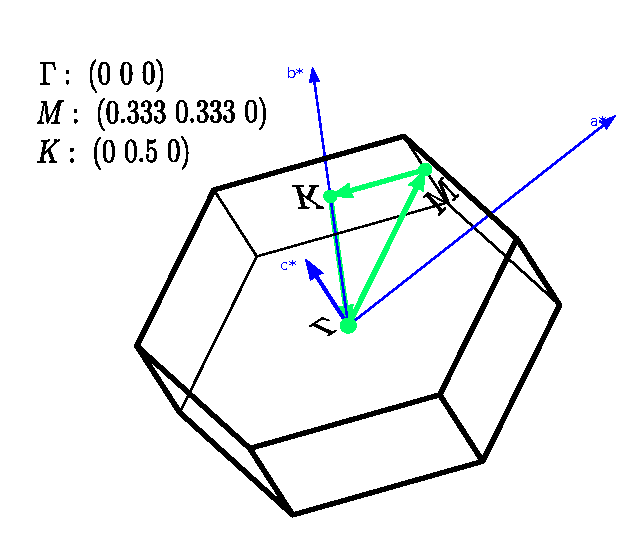
\epsfig{file=figMet/espacioK2.eps, width=5.0cm,height=5.0cm }
            	\caption{Primera zona de Brillouin con sus puntos especiales.}
            \end{figure}
				

	   %
	   \pause
	   \column{0.6\textwidth}
	   		\begin{itemize}
	   			\item $K-\Gamma-M-K$ para el PtSe\textsubscript{2} y PtS\textsubscript{2}
	   			\pause
	   			\vspace{0.7cm}
	   			\item $\Gamma-M-K-\Gamma$ para el VSe\textsubscript{2} y VS\textsubscript{2}
	   		\end{itemize}
	\end{columns}
}
\endinput

	\subsection{Resultados de la simulaciones}
\subsubsection{Materiales sin defectos}
\frame{
	\frametitle{Materiales sin defectos}
	\framesubtitle{PtSe\textsubscript{2} y PtS\textsubscript{2}}
	\begin{table}[!hbt]
		\centering
		\begin{tabular}{|c||c|c|c|}
			\hline
			Material & Celda & Constante de Red (\AA) &Magnetizaci\'on\\
			\hline
			\hline
			PtSe\textsubscript{2} & 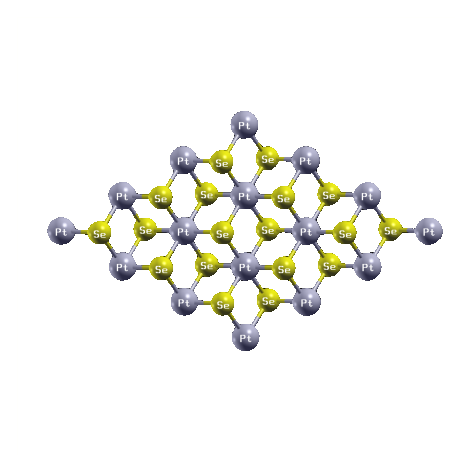
\epsfig{file=figRes/PtSe2/est/est1.eps, scale=0.3}& $3.7610$&$0\mu_{B}/celda$ \\
			\hline
			PtS\textsubscript{2} & 	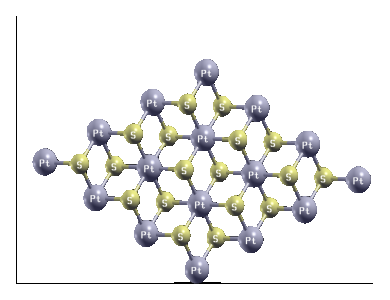
\epsfig{file=figRes/PtS2/parCelU.eps, scale=0.3}& $3.5785$&$0\mu_{B}/celda$\\
			\hline
		\end{tabular}
	\end{table}
}

\frame{
	\frametitle{Materiales sin defectos}
	\framesubtitle{VSe\textsubscript{2} y VS\textsubscript{2}}
	\begin{table}[!hbt]
		\centering
		\begin{tabular}{|c||c|c|c|}
			\hline
			Material & Celda &Constante de Red (\AA)& Magnetizaci\'on \\
			\hline
			\hline
			VSe\textsubscript{2} & 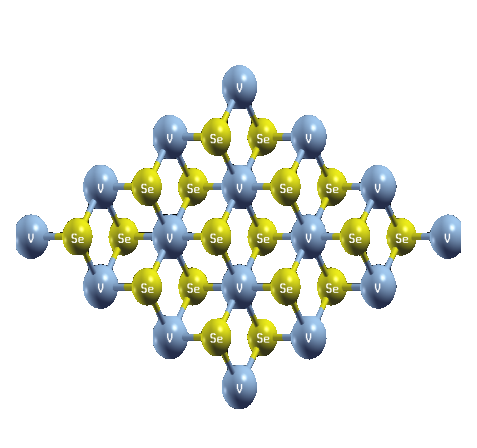
\epsfig{file=figRes/VSe2/par.png.eps, scale=0.3}&$3.3403$ & $0.62\mu_{B}/celda$\\
			\hline
			VS\textsubscript{2} & 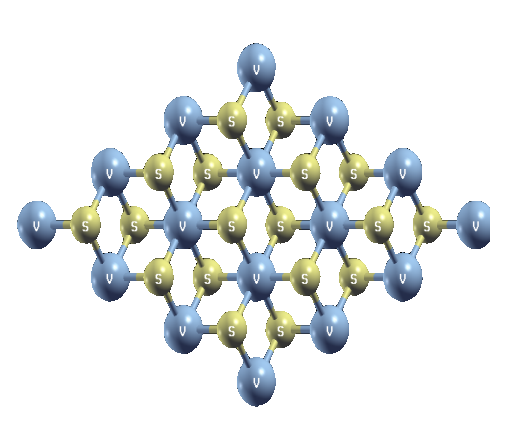
\epsfig{file=figRes/VS2/par.eps, scale=0.3}&$3.1939$ &$0.55\mu_{B}/celda$\\
			\hline
		\end{tabular}
	\end{table}
}
\frame{
	\frametitle{VSe\textsubscript{2}}
	\framesubtitle{Diagrama de Bandas y Densidad de estados}
	\begin{figure}
		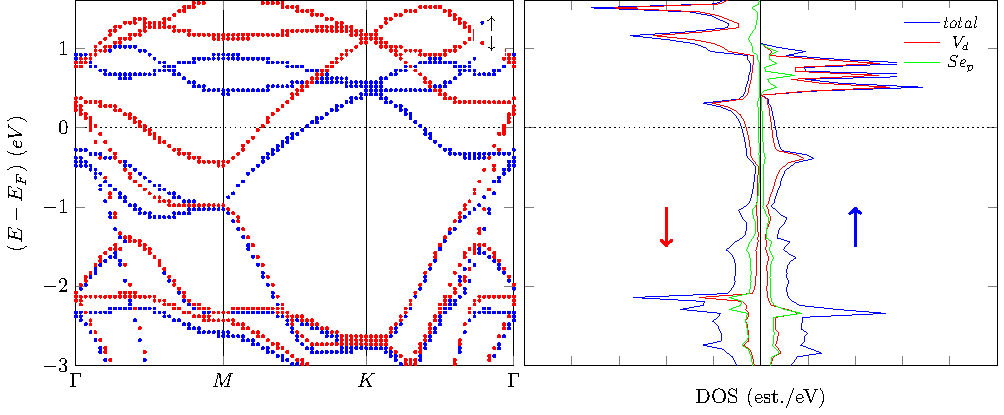
\includegraphics[scale=0.6]{figRes/VSe2/bandas/celU/nosoc/bandasDOSnoSoc.pdf}
		\label{Sim:fig:bandnoSocVse2}
		\caption{Diagrama de bandas y densidad de estados del VSe\textsubscript{2} sin efecto spin-\'orbita.}
	\end{figure}	
}
\frame{
	\frametitle{VS\textsubscript{2}}
	\framesubtitle{Diagrama de Bandas y Densidad de estados}
	\begin{figure}
		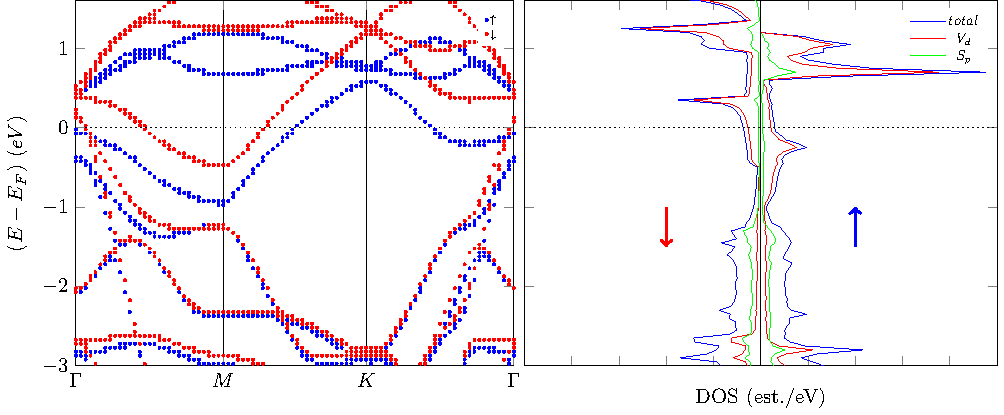
\includegraphics[scale=0.6]{figRes/VS2/celdaU/estructura electronica/noSOC/bandasDOSnoSoc.pdf}
		\label{Sim:fig:bandnoSocVs2}
		\caption{Diagrama de bandas y densidad de estados del VS\textsubscript{2} sin efecto spin-\'orbita.}
	\end{figure}	
}
\frame{
	\frametitle{VSe\textsubscript{2}}
	\framesubtitle{Densidad de spin}
	\begin{figure}[!hbt]
		\centering
		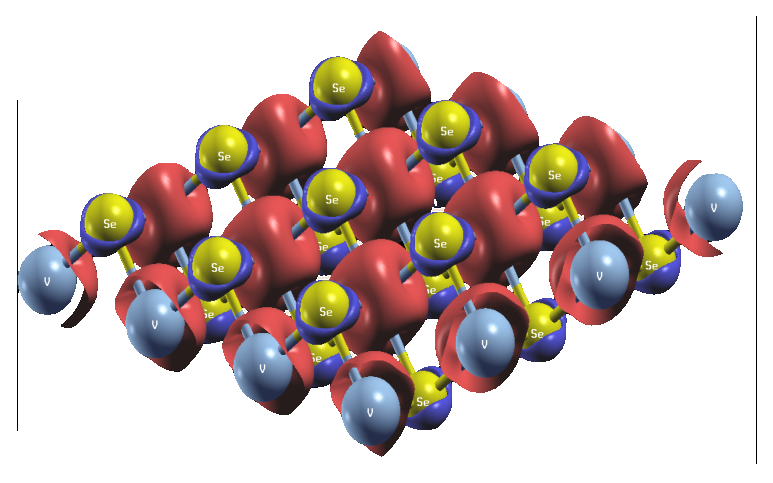
\epsfig{file=figRes/VSe2/vse2magz.eps, scale=0.5}
		\caption[Distribuci\'on de spin en VSe\textsubscript{2}]{Distribuci\'on  de spin en el VSe\textsubscript{2}.}
		\label{Sim:fig:distmagnVse2}
	\end{figure}
}
\frame{
	\frametitle{VS\textsubscript{2}}
	\framesubtitle{Densidad de spin}
	\begin{figure}[!hbt]
		\centering
		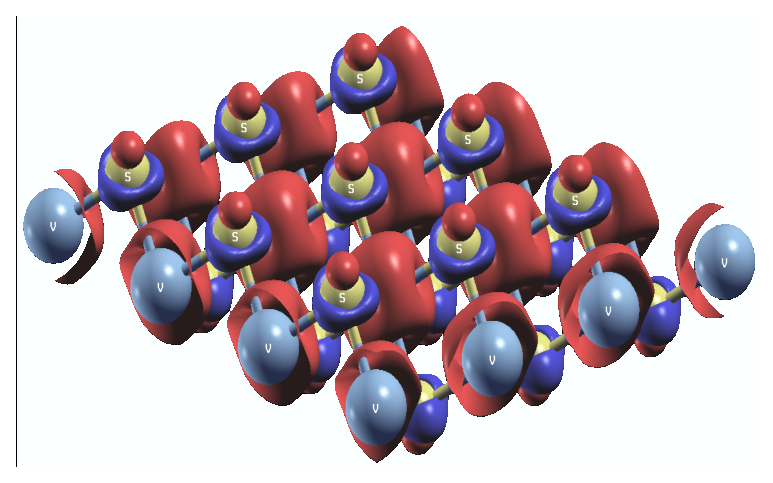
\epsfig{file=figRes/VS2/vs2magz.eps, scale=0.5}
		\caption[Densidad de spin en el VS\textsubscript{2}.]{Distribuci\'on  de spin en el VS\textsubscript{2}.}
		\label{Sim:fig:distmagnVs2}
	\end{figure}
}
\subsubsection{Estudio de vacancia de metal de transici\'on}
\frame{
    \frametitle{Vacancia de Platino en PtSe\textsubscript{2} y PtS\textsubscript{2}}
	\begin{table}[!hbt]
		\centering
		\begin{tabular}{|c||c|c|}
			\hline
			Material & Celda & Momento magn\'etico \\
			\hline
			\hline
			PtSe\textsubscript{2} &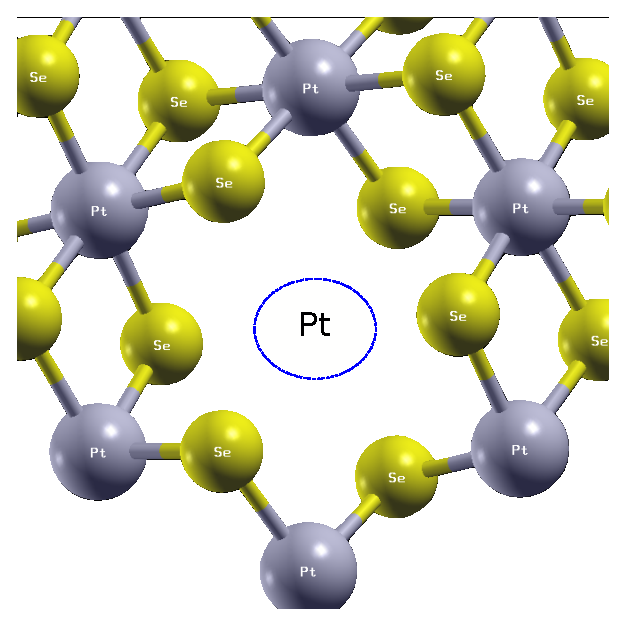
\epsfig{file=figRes/PtSe2/VacanciaPt.eps, scale=0.3}& $2.37\mu_{B}/celda$\\
			\hline
			PtS\textsubscript{2} &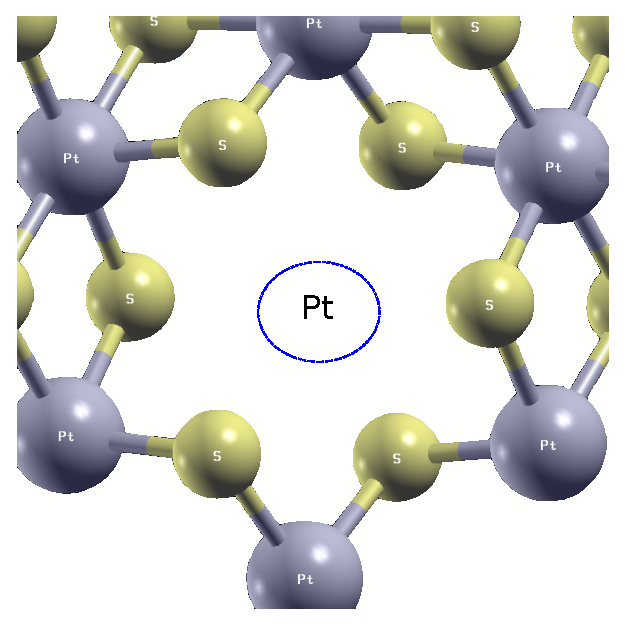
\epsfig{file=figRes/PtS2/VacanciaPt.eps, scale=0.3}& $2.63\mu_{B}/celda$\\
			\hline
		\end{tabular}
	\end{table}
}
\frame{
	\frametitle{Vacancia de Platino en PtSe\textsubscript{2} y PtS\textsubscript{2}}
	\framesubtitle{Densidad de carga}
	
	\begin{figure}[!hbt]
		\centering
		\subfigure[PtSe\textsubscript{2}]{
			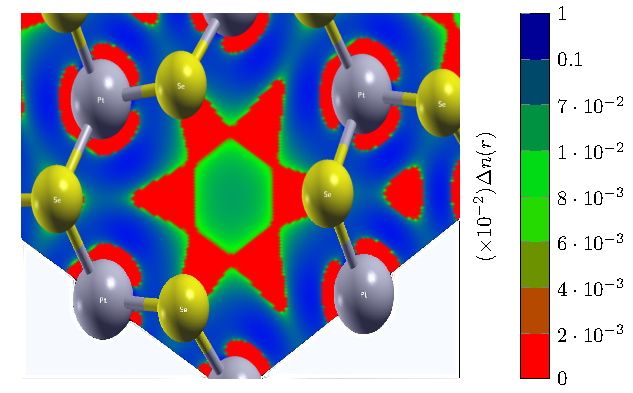
\includegraphics[scale=0.45]{figRes/PtSe2/densidades/densPos/densidadpos.pdf}
			\label{Sim:fig:cargavacPtse2}
		}
		\subfigure[PtS\textsubscript{2}]{
			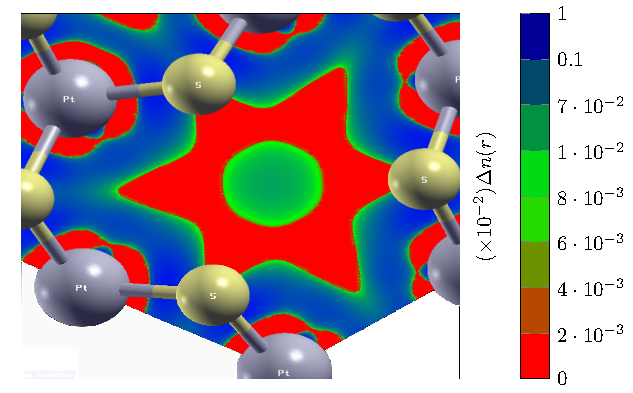
\includegraphics[scale=0.45]{figRes/PtS2/def/densidades/denspos/densidadpos.pdf}
			\label{Sim:fig:cargavacPts2}
		}
		\caption[Distribuci\'on de carga en alrededor de la vacancia de platino en PtSe\textsubscript{2} y PtSe\textsubscript{2}.]{Distribuci\'on de carga alrededor de la vacancia de platino en PtSe\textsubscript{2} (\ref{Sim:fig:cargavacPtse2}), y en PtS\textsubscript{2} (\ref{Sim:fig:cargavacPtse2}).}
		\label{Sim:fig:cargavac}	
	\end{figure}
}

\frame{
	\frametitle{Vacancia de Platino en PtSe\textsubscript{2} y PtS\textsubscript{2}}
	\framesubtitle{Diagrama de bandas y densidad de estados del PtSe\textsubscript{2}}
	
	\begin{figure}[!hbt]
		\centering
		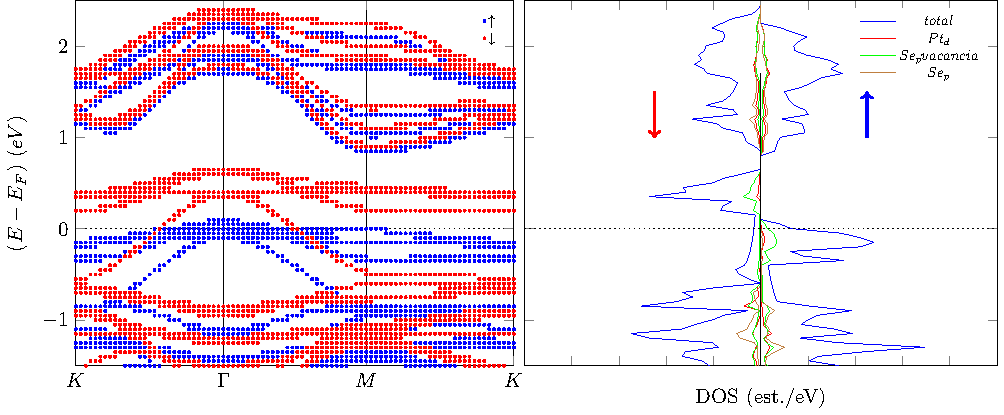
\includegraphics[scale=0.7]{figRes/PtSe2/def/bandas/nosoc/bandasDOSnoSoc.pdf}
		\caption[Diagrama de bandas y densidad de estados del PtSe\textsubscript{2} con vacancia de Platino.]{Diagrama de bandas y densidad de estados sin incluir el efecto de spin \'orbita en el PtSe\textsubscript{2}.}
		\label{Sim:fig:bandDefPtse2noSOC}
	\end{figure}
}
\frame{
	\frametitle{Vacancia de Platino en PtSe\textsubscript{2} y PtS\textsubscript{2}}
	\framesubtitle{Diagrama de bandas y densidad de estados del PtS\textsubscript{2}}
	\begin{figure}[!hbt]
		\centering
		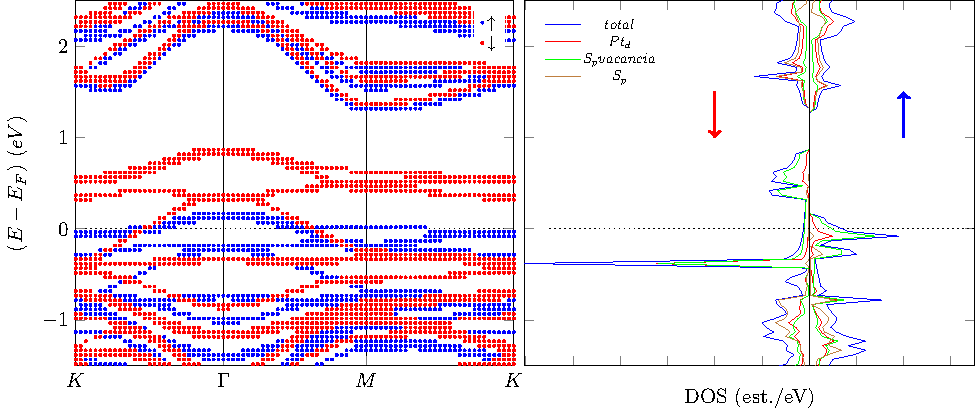
\includegraphics[scale=0.7]{figRes/PtS2/def/bandas/nosoc/bandasDOSnoSoc.pdf}
		\caption[Diagrama de bandas y densidad de estados del PtS\textsubscript{2} con una vacancia de Platino.]{Diagrama de bandas y densidad de estados del PtS\textsubscript{2}.  }
		\label{Sim:fig:noSOCpts2def}
	\end{figure}
}
\frame{
	\frametitle{Vacancia de Platino en PtSe\textsubscript{2} y PtS\textsubscript{2}}
	\framesubtitle{Densidad de carga y de spin en PtSe\textsubscript{2}}
	\begin{figure}[!hbt]
		\centering
		\subfigure[densidad de carga]{
			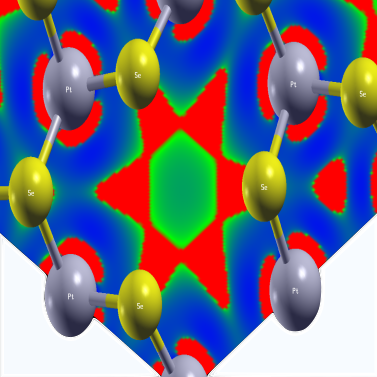
\epsfig{file=figRes/PtSe2/def/ptse2_carga, scale=0.6}
			\label{Sim:fig:CargaVacPtse2}
		}
		\subfigure[densidad de spines]{
			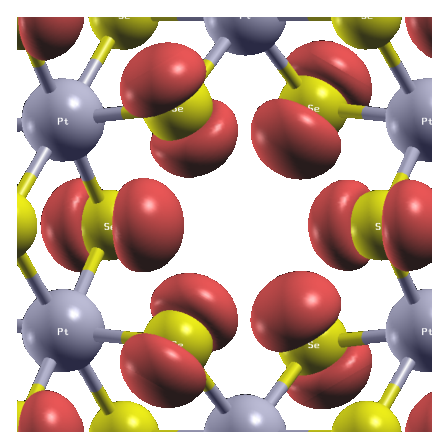
\epsfig{file=figRes/PtSe2/def/ptse2_magz, scale=0.6}
			\label{Sim:fig:MagzVacPtse2}
		}
		\caption[Iso superficies de la densidad de carga y de spin en el PtSe\textsubscript{2} con vacancia de Platino.]{Isosuperficies de la densidad de carga (\ref{Sim:fig:CargaVacPtse2}) y la densidad de spines (\ref{Sim:fig:MagzVacPtse2} del PtSe\textsubscript{2} con un valor de $0.001 e/\AA^3$. }
	\end{figure}
}

\frame{
	\frametitle{Vacancia de Platino en PtSe\textsubscript{2} y PtS\textsubscript{2}}
	\framesubtitle{Densidad de carga y de spin en PtS\textsubscript{2}}
	\begin{figure}[!hbt]
		\centering
		\subfigure[densidad de carga]{
			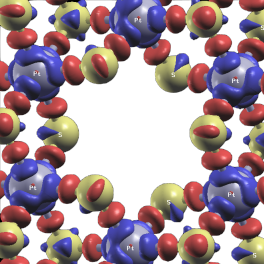
\epsfig{file=figRes/PtS2/def/densidades/pts2_carga, scale=0.6}
			\label{Sim:fig:CargaVacPts2}
		}
		\subfigure[densidad de spines]{
			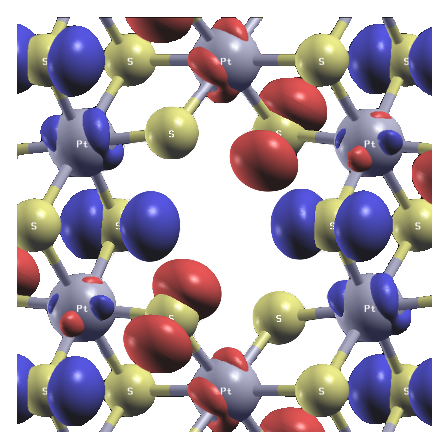
\epsfig{file=figRes/PtS2/def/densidades/pts2_magz, scale=0.6}
			\label{Sim:fig:MagzVacPts2}
		}
		\caption[Iso superficies de la densidad de carga y de spin en el PtS\textsubscript{2} con vacancia de Platino.]{Isosuperficies de la densidad de carga (\ref{Sim:fig:CargaVacPts2}) y la densidad de spines (\ref{Sim:fig:MagzVacPts2} del PtS\textsubscript{2} con un valor de $0.001 e/\AA^3$. }
	\end{figure} 
}
\frame{
	\frametitle{Vacancia de Vanadio en VSe\textsubscript{2} y VS\textsubscript{2}}
	\begin{table}[!hbt]
		\centering
		\begin{tabular}{|c||c|c|}
			\hline
			Material & Celda & Momento magn\'etico \\
			\hline
			\hline
			VSe\textsubscript{2} & 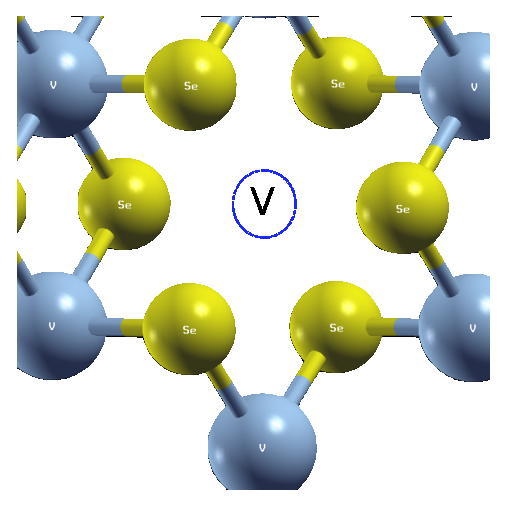
\epsfig{file=figRes/VSe2/def/vacVse2_def, scale=0.34}& $0.48\mu_{B}/celda$\\
			\hline
			VS\textsubscript{2} & 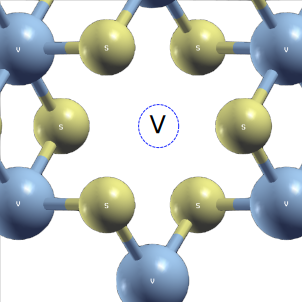
\epsfig{file=figRes/VS2/def/vs2_def, scale=0.34}& $0.76\mu_{B}/celda$\\
			\hline
		\end{tabular}
	\end{table}
}

\frame{
	\frametitle{Vacancia de Vanadio en VSe\textsubscript{2} y VS\textsubscript{2}}
	\framesubtitle{Densidad de carga}
	
	\begin{figure}[!hbt]
		\centering
		\subfigure[VSe\textsubscript{2}]{
			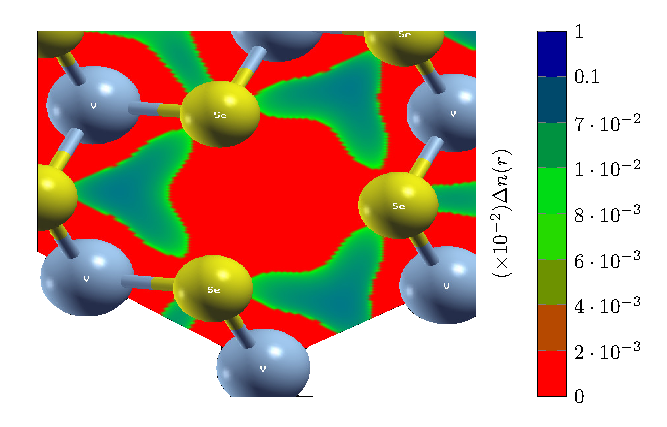
\epsfig{file=figRes/VSe2/def/densidad/densPos/densidadpos, scale=0.45}
			\label{Sim:fig:cargavacVSe2}
		}
		\subfigure[VS\textsubscript{2}]{
			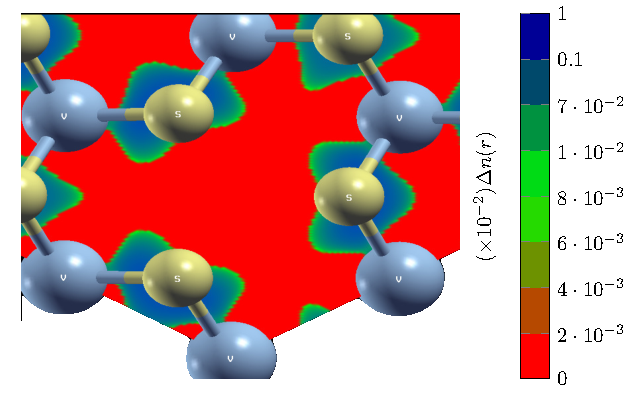
\epsfig{file=figRes/VS2/def/dens/densPos/densidadpos, scale=0.45}
			\label{Sim:fig:cargavacVS2}
		}
		\caption[densidad de carga en el VSe\textsubscript{2} yVS\textsubscript{2}]{densidad de carga en la regi\'on de la vacancia en el VSe\textsubscript{2} y VS\textsubscript{2} visualizada con XcrySDen }
		\label{Sim:fig:cargavacV}	
	\end{figure}
}
\frame{
	\frametitle{Vacancia de Vanadio en VSe\textsubscript{2} y VS\textsubscript{2}}
	\framesubtitle{Diagrama de bandas y densidad de estados del VSe\textsubscript{2}}
	
	\begin{figure}[!hbt]
		\centering
		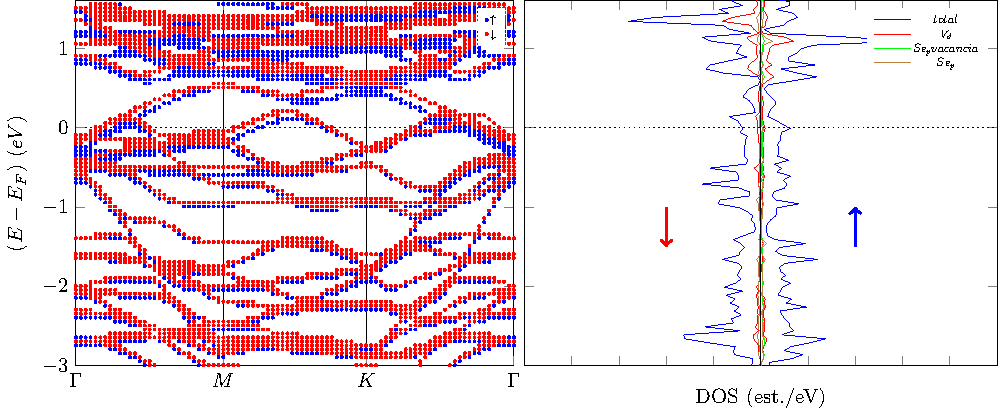
\includegraphics[width=10cm, height=5cm]{figRes/VSe2/def/bandas/nosoc/bandasDOSnoSoc.pdf}
		\caption[diagrama de bandas y densidad de estados del VSe\textsubscript{2} con vacancia de Vanadio.]{Diagrama de bandas y la densidad de estados para el VSe\textsubscript{2}.} 
		\label{Sim:fig:VSe2noSOCcavband}
	\end{figure}
}
\frame{
	\frametitle{Vacancia de Vanadio en VSe\textsubscript{2} y VS\textsubscript{2}}
	\framesubtitle{Diagrama de bandas y densidad de estados del VS\textsubscript{2}}
	\begin{figure}[!hbt]
		\centering
		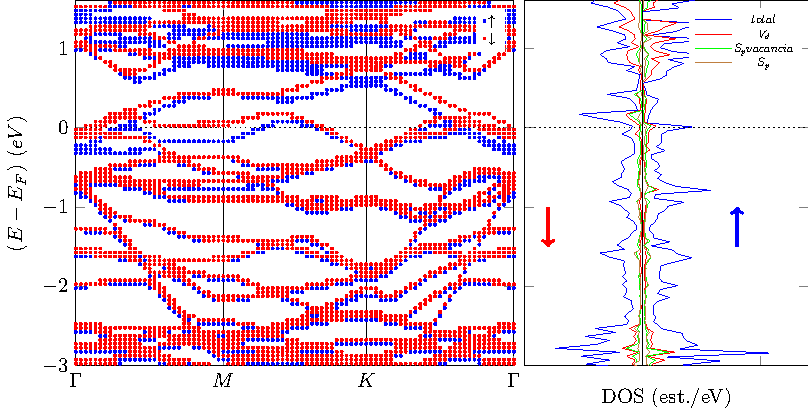
\includegraphics[scale=0.7]{figRes/VS2/def/bandas/nosoc/bandasDOSnoSoc.pdf}
		\caption[Diagrama de bandas  y densidad de estados en el VS\textsubscript{2} con vacancia de Vanadio]{Diagrama de bandas y Densidad de Estados del  VS\textsubscript{2}.}
		\label{Sim:fig:VacVS2bandas}
	\end{figure}
}
\frame{
	\frametitle{Vacancia de Vanadio en VSe\textsubscript{2} y VS\textsubscript{2}}
	\framesubtitle{Densidad de carga en VSe\textsubscript{2} y VS\textsubscript{2}}
	\begin{figure}[!hbt]
		\centering
		\subfigure[VSe\textsubscript{2}]{
			
\epsfig{file=figRes/VSe2/def/densidad/vse2_carga_vac.eps, scale=0.6}
			\label{Sim:fig:cargaVacVSe2}
		}
		\subfigure[VS\textsubscript{2}]{
			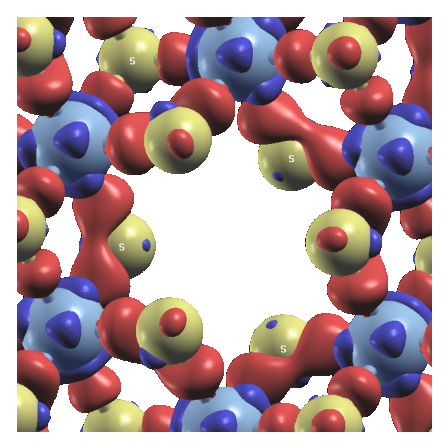
\epsfig{file=figRes/VS2/def/dens/vs2_carga_vac.eps, scale=0.6}
			\label{Sim:fig:cargaVacVS2}
			
		}
		\caption[Densidad de electrones en el VSe\textsubscript{2} y VS\textsubscript{2} con vacancia de Vanadio.]{Iso superficies de la densidad de carga con  un valor de $\pm 0.001 e/\AA^3$}
		\label{Sim:fig:cargaVac}
	\end{figure}
}

\frame{
	\frametitle{Vacancia de Vanadio en VSe\textsubscript{2} y VS\textsubscript{2}}
	\framesubtitle{Densidad de spin en VSe\textsubscript{2} y VS\textsubscript{2}}
	
	\begin{figure}[!hbt]
		\centering
		\subfigure[VSe\textsubscript{2}]{
			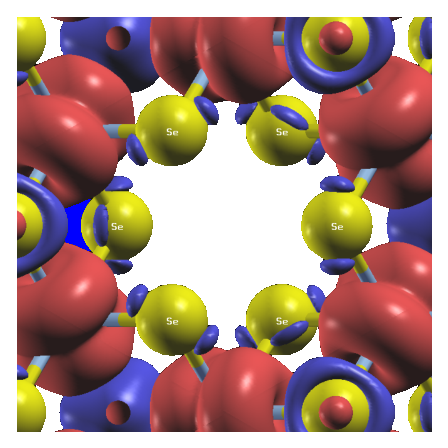
\epsfig{file=figRes/VSe2/def/densidad/vse2_magz.eps, scale=0.6}
			\label{Sim:fig:magnVacVSe2}
		}
		\subfigure[VS\textsubscript{2}]{
			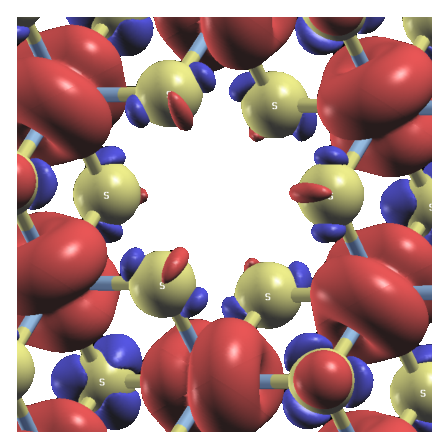
\epsfig{file=figRes/VS2/def/dens/vs2_magz.eps, scale=0.6}
			\label{Sim:fig:magnVacVS2}
			
		}
		\caption[Densidad de spin en el VSe\textsubscript{2} y VS\textsubscript{2} con vacancia de Vanadio.]{Iso superficies de la densidad de spines con  un valor de $\pm 0.0002 e/\AA^3$}
		\label{Sim:fig:magzVacV}
	\end{figure}
}
\subsubsection{Efectos de la deformaci\'on mec\'anica en la magnetizaci\'on}
\frame{
	\frametitle{Deformaci\'on isotr\'opica en VSe\textsubscript{2} y VS\textsubscript{2}}
	\framesubtitle{Magnetizaci\'on}
	\begin{figure}[!hbt]
		\centering
		\subfigure[VSe\textsubscript{2}]{
			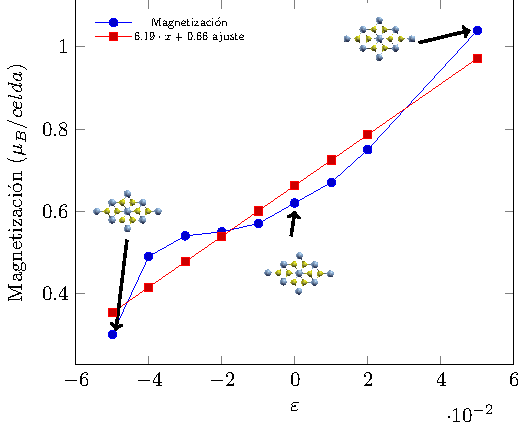
\includegraphics[scale=0.55]{figRes/VSe2/str/isotropico/magn.pdf}
			\label{Sim:fig:strVSe2Iso}
		}
		\subfigure[VS\textsubscript{2}]{
			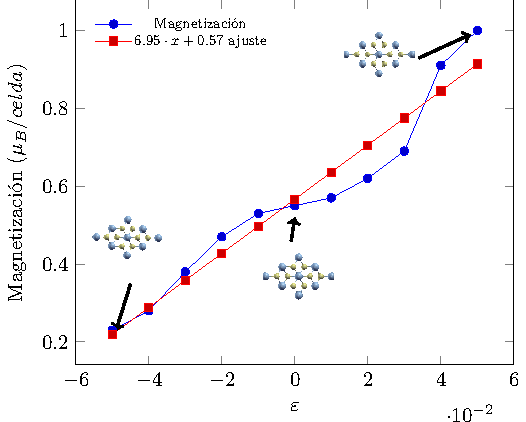
\includegraphics[scale=0.55]{figRes/VS2/str/isotropico/magn.pdf}
			\label{Sim:fig:strVS2Iso}
		}
		\caption[Magnetizaci\'on del VSe\textsubscript{2} y VS\textsubscript{2} en funci\'on de una deformaci\'on isotr\'opica. ]{Gr\'aficas de la magnetizaci\'on en funci\'on de la deformaci\'on isotr\'opica en VSe\textsubscript{2} y VS\textsubscript{2} mostrando el ajuste lineal de los datos.}
		\label{Sim:fig:MgnVx2Iso}
	\end{figure}
}
\frame{
	\frametitle{Deformaci\'on isotr\'opica en VSe\textsubscript{2} y VS\textsubscript{2}}
	\framesubtitle{An\'alisis de distancias}
	\begin{figure}[!hbt]
		\centering
		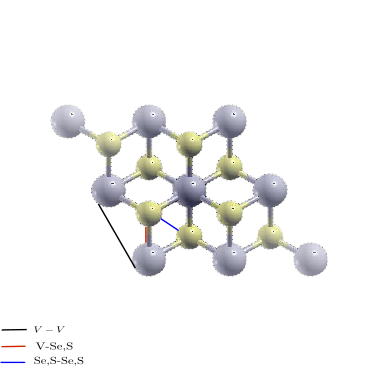
\epsfig{file=figRes/compIso,scale=0.5}
		\caption[ Distancias entre \'atomos   VSe\textsubscript{2} y VS\textsubscript{2} utilizados para el estudio de una deformaci\'on isotr\'opica]{Distancias entre \'atomos en el VSe\textsubscript{2} y  VS\textsubscript{2} en donde las esferas grises representran el vanadio y las amarillas El Azufre o Selenio.}
		\label{Sim:fig:disVX2Iso}
	\end{figure}
}
\frame{
	\frametitle{Deformaci\'on isotr\'opica en VSe\textsubscript{2} y VS\textsubscript{2}}
	\framesubtitle{Cambio en distancia entre \'atomo de Azufre o Selenio y Vanadio}
	\begin{figure}[!hbt]
		\centering
		\subfigure[VSe\textsubscript{2}]{
			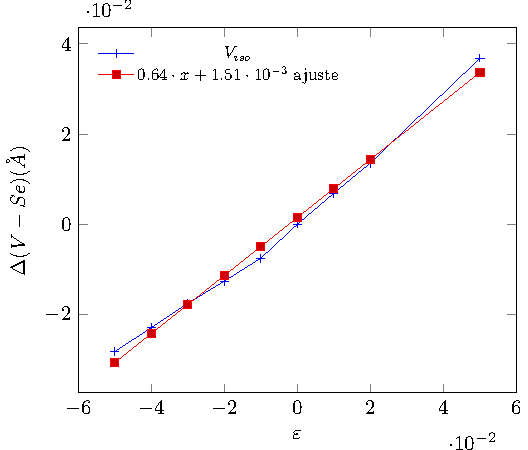
\includegraphics[scale=0.55]{figRes/VSe2/str/isotropico/dVS.pdf}
			\label{Sim:fig:DVSVSe2Iso}
		}
		\subfigure[VS\textsubscript{2}]{
			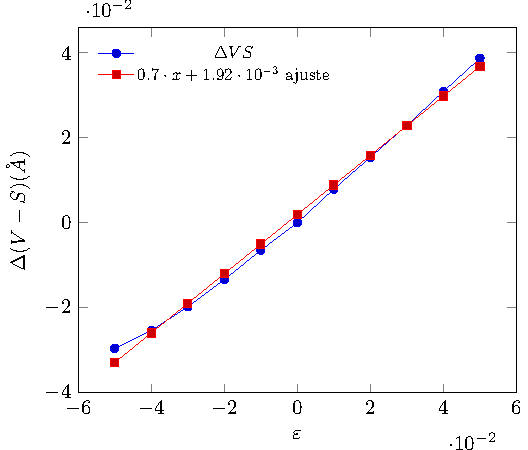
\includegraphics[scale=0.55]{figRes/VS2/str/isotropico/dVS.pdf}
			\label{Sim:fig:DVSVS2Iso}
		}
		\caption[Cambio en la distancia entre \'atomos de Selenio o Azufre en  VSe\textsubscript{2} y VS\textsubscript{2} en funci\'on de una deformaci\'on isotr\'opica. ]{Cambio en la distancia entre dos \'atomos de Selenio en VSe\textsubscript{2} y Azufre en VS\textsubscript{2}.}
		\label{Sim:fig:DVSVx2Iso}
	\end{figure}
}
\frame{
	\frametitle{Deformaci\'on isotr\'opica en VSe\textsubscript{2} y VS\textsubscript{2}}
	\framesubtitle{magnetizaci\'on de cada \'atomo}
	\begin{figure}[!hbt]
		\centering
		\subfigure[VSe\textsubscript{2}]{
			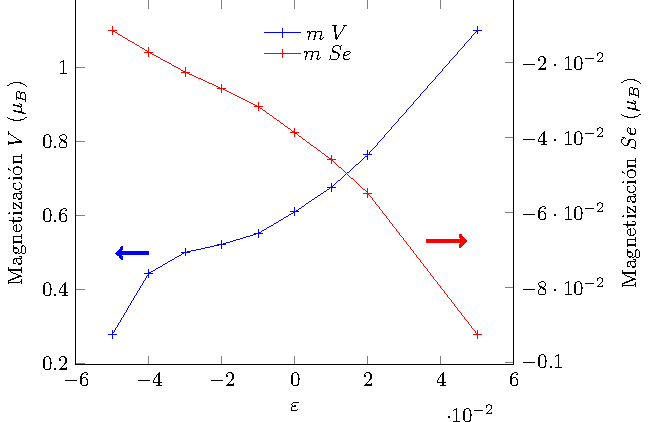
\includegraphics[scale=0.4]{figRes/VSe2/str/isotropico/CompMag.pdf}
			\label{Sim:fig:cmagVse2I}	
		}
		\subfigure[VS\textsubscript{2}]{
			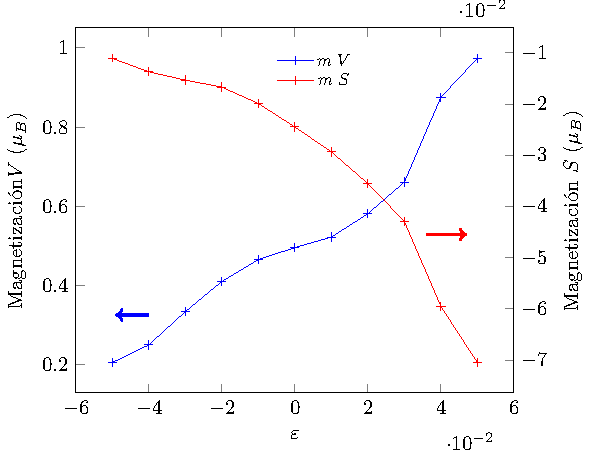
\includegraphics[scale=0.4]{figRes/VS2/str/isotropico/CompMag.pdf}
			\label{Sim:fig:cmagVs2I}	
		}
		\caption{magnetizaci\'on del \'atomo de vanadio y selenio o Azufre en el VSe2 (\ref{Sim:fig:cmagVse2I}) y VS\textsubscript{2} (\ref{Sim:fig:cmagVs2I}) bajo una deformaci\'on isotr\'opica.}
		\label{Sim:fig:cmagVX2I}
	\end{figure} 
}
\frame{
	\frametitle{Deformaci\'on anisotr\'opica en VSe\textsubscript{2} y VS\textsubscript{2}}
	\framesubtitle{Magnetizaci\'on}
	\begin{figure}[!hbt]
		\centering
		\subfigure[VSe\textsubscript{2}]{
			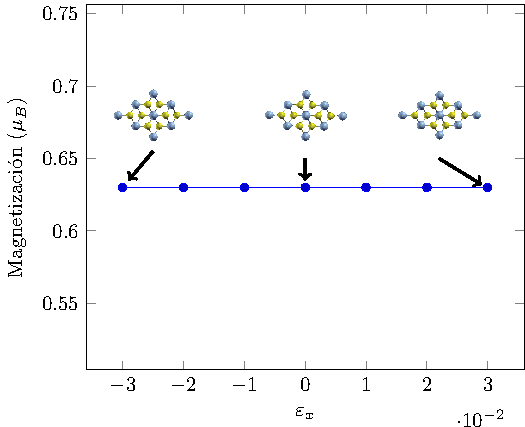
\includegraphics[scale=0.55]{figRes/VSe2/str/anisotropico/magn.pdf}
			\label{Sim:fig:strVSe2anis}
		}
		\subfigure[VS\textsubscript{2}]{
			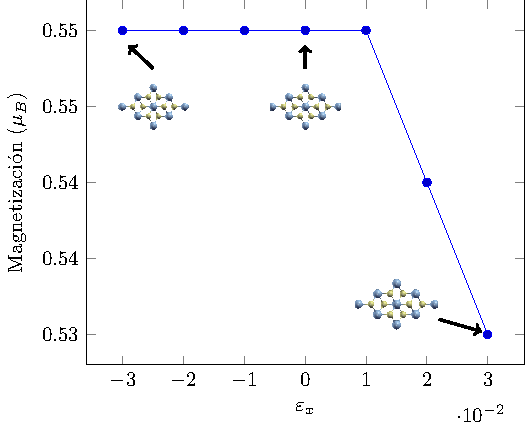
\includegraphics[scale=0.55]{figRes/VS2/str/anisotropico/magn.pdf}
			\label{Sim:fig:strVS2Anis}
		}
		\caption[magnetizaci\'on del VSe\textsubscript{2} y VS\textsubscript{2} bajo una deformaci\'on anisotr\'opica.]{Gr\'aficas de la magnetizaci\'on en funci\'on de la deformaci\'on anisotr\'opica en VSe\textsubscript{2} y VS\textsubscript{2}.}
		\label{Sim:fig:MgnVx2Anis}
	\end{figure}
}
\frame{
	\frametitle{Deformaci\'on anisotr\'opica en VSe\textsubscript{2} y VS\textsubscript{2}}
	\framesubtitle{An\'alisis de distancias}
	\begin{figure}[!hbt]
		\centering
		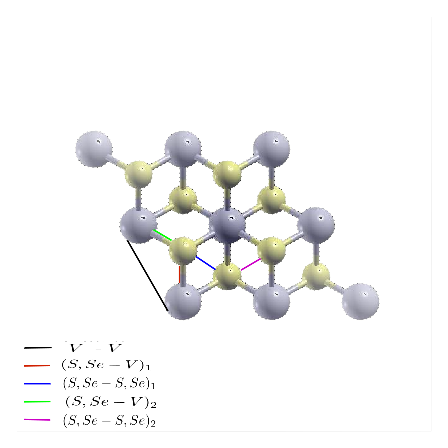
\epsfig{file=figRes/compAnis.eps,scale=0.6}
		\caption[Distancias entre \'atomos   VSe\textsubscript{2} y VS\textsubscript{2} utilizados para el estudio de una deformaci\'on aniisotr\'opica.]{Distancias entre \'atomos en el VSe\textsubscript{2} y  VS\textsubscript{2} en la deformaci\'on anisotr\'opica, las esferas grises representan el vanadio y las amarillas El Azufre o Selenio.}
		\label{Sim:fig:disVX2Anis}
	\end{figure}
}
\frame{
	\frametitle{Deformaci\'on anisotr\'opica en VSe\textsubscript{2} y VS\textsubscript{2}}
	\framesubtitle{Cambio en distancia entre \'atomo de Azufre o Selenio y Vanadio}
	\begin{figure}[!hbt]
		\centering
		\subfigure[VSe\textsubscript{2}]{
			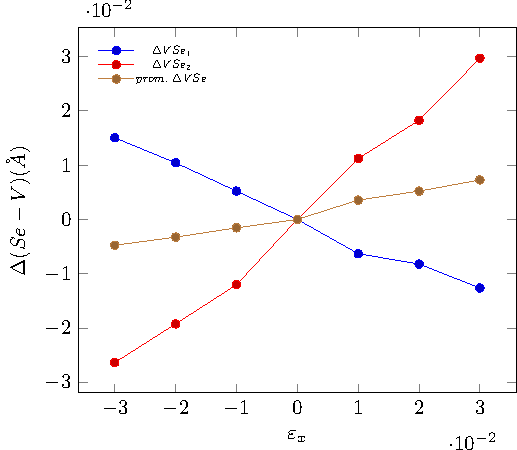
\includegraphics[scale=0.55]{figRes/VSe2/str/anisotropico/CompdVS.pdf}
			\label{Sim:fig:compdSVVse2}	
		}
		\subfigure[VS\textsubscript{2}]{
			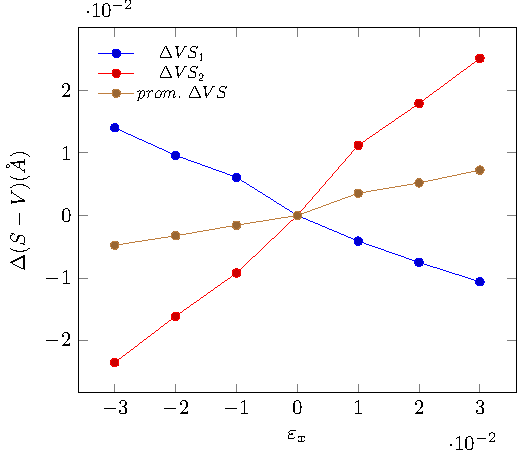
\includegraphics[scale=0.55]{figRes/VS2/str/anisotropico/CompdVS.pdf}
			\label{Sim:fig:compdSVVs2}	
		}
		\caption{variaci\'on de las distancias entre \'atomos de Selenio en el VSe\textsubscript{2} y de Azufre en VS\textsubscript{2}.}
		\label{Sim:fig:compdSVVX2}
	\end{figure}
}
\frame{
	\frametitle{Deformaci\'on anisotr\'opica en VSe\textsubscript{2} y VS\textsubscript{2}}
	\framesubtitle{magnetizaci\'on de cada \'atomo}
	\begin{figure}[!hbt]
		\centering
		\subfigure[VSe\textsubscript{2}]{
			\includegraphics[scale=0.4]{figRes/VSe2/str/anisotropico/CompMag.pdf}
			\label{Sim:fig:cmagVse2}	
		}
		\subfigure[VS\textsubscript{2}]{
			\includegraphics[scale=0.4]{figRes/VS2/str/anisotropico/CompMag.pdf}
			\label{Sim:fig:cmagVs2}	
		}
		\caption{magnetizaci\'on del \'atomo de vanadio y selenio o Azufre en el Vse2 (\ref{Sim:fig:cmagVse2}) y VS\textsubscript{2} (\ref{Sim:fig:cmagVs2}) bajo una deformaci\'on anisotr\'opica.}
		\label{Sim:fig:cmagVX2}
	\end{figure} 
}
%================================================================================================================
\frame{
	\frametitle{Deformaci\'on isotr\'opica en PtSe\textsubscript{2} y PtS\textsubscript{2}}
	\framesubtitle{Magnetizaci\'on}
	\begin{figure}[!hbt]
		\centering
		\subfigure[PtSe\textsubscript{2}]{
			\includegraphics[scale=0.5]{figRes/PtSe2/str/isotropico/magn.pdf}
			\label{Sim:fig:magnPtSe2}
		}
		\subfigure[PtS\textsubscript{2}]{
			\includegraphics[scale=0.5]{figRes/PtS2/str/isotropico/magn.pdf}
			\label{Sim:fig:magnPtS2}
			
		}
		\caption{Magnetizaci\'on en funci\'on de una deformaci\'on isotr\'opica en PtSe\textsubscript{2} y PtS\textsubscript{2} con una vacancia de Platino}
		\label{Sim:fig:magnPtX2}
	\end{figure}
}
\frame{
	\frametitle{Deformaci\'on isotr\'opica en PtSe\textsubscript{2} y PtS\textsubscript{2}}
	\framesubtitle{An\'alisis de distancias}
	\begin{figure}[htbp]
		\centering
		\epsfig{file=figRes/compIsoDef, scale=0.3}
		\caption{Distancias entre \'atomos que se utilizan para estudiar una desinformación isotrópica, las esferas grises representan los \'atomos de Platino y las amarillas a \'atomos de Selenio o  azufre. }
		\label{Sim:fig:defIsoPtX2}
	\end{figure}
}
\frame{
	\frametitle{Deformaci\'on isotr\'opica en PtSe\textsubscript{2} y PtS\textsubscript{2}}
	\framesubtitle{Cambio en distancia entre \'atomos de Azufre o Selenio}
	\begin{figure}[!hbt]
		\centering
		\subfigure[PtSe\textsubscript{2}]{
			\includegraphics[scale=0.45]{figRes/PtSe2/str/isotropico/CompdS.pdf}
			\label{Sim:fig:compdSePPtSe2}
		}
		\subfigure[PtS\textsubscript{2}]{
			\includegraphics[scale=0.45]{figRes/PtS2/str/isotropico/CompdS.pdf}
			\label{Sim:fig:compdSePPtS2}
		}
		\caption{Comparaci\'on del cambio entre \'atomos de Selenio en el PtSe\textsubscript{2} (\ref{Sim:fig:compdSePPtSe2}) y de Azufre en PtS\textsubscript{2} (\ref{Sim:fig:compdSePPtS2}.)
		}
		\label{Sim:fig:compdSePPtX2}
	\end{figure}
}
\frame{
	\frametitle{Deformaci\'on isotr\'opica en PtSe\textsubscript{2} y PtS\textsubscript{2}}
	\framesubtitle{magnetizaci\'on de cada \'atomo}
	\begin{figure}[!hbt]
		\centering
		\subfigure[PtSe\textsubscript{2}]{
			\includegraphics[scale=0.45]{figRes/PtSe2/str/isotropico/CompMagn.pdf}
			\label{Sim:fig:magnCptse2iso}
		}
		\subfigure[PtS\textsubscript{2}]{
			\includegraphics[scale=0.45]{figRes/PtS2/str/isotropico/CompMagn.pdf}
			\label{Sim:fig:magnCpts2iso}
		}
		\caption{magnetizaci\'on correspondiente a cada \'atomo de PtSe\textsubscript{2} yPtS\textsubscript{2} sujetos a una deformaci\'on isotr\'opica}
		\label{Sim:fig:magnCptx2iso}
	\end{figure}
}
\frame{
	\frametitle{Deformaci\'on anisotr\'opica en PtSe\textsubscript{2} y PtS\textsubscript{2}}
	\framesubtitle{Magnetizaci\'on}
	\begin{figure}[!hbt]
		\centering
		\subfigure[PtSe\textsubscript{2}]{
			\includegraphics[scale=0.5]{figRes/PtSe2/str/anisotropico/magn.pdf}
			\label{Sim:fig:magnPtSe2anis}
		}
		\subfigure[PtS\textsubscript{2}]{
			\includegraphics[scale=0.5]{figRes/PtS2/str/anisotropico/magn.pdf}
			\label{Sim:fig:magnPtS2anis}
			
		}
		\caption{Magnetizaci\'on en funci\'on de una deformaci\'on isotr\'opica en PtSe\textsubscript{2} y PtS\textsubscript{2} con una vacancia de Platino}
		\label{Sim:fig:magnPtX2anis}
		
	\end{figure}
}
\frame{
	\frametitle{Deformaci\'on anisotr\'opica en PtSe\textsubscript{2} y PtS\textsubscript{2}}
	\framesubtitle{An\'alisis de distancias}
	\begin{figure}[!hbt]
		\centering
		\includegraphics[scale=0.3]{figRes/compAnisDef.eps}
		\caption{Distancias entre \'atomos que se utilizan para estudiar una desinformación anisotr\'opica, las esferas grises representan los \'atomos de Platino y las amarillas a \'atomos de Selenio o  azufre. }
		\label{Sim:fig:defAnisPtX2}
	\end{figure}
}
\frame{
	\frametitle{Deformaci\'on anisotr\'opica en PtSe\textsubscript{2} y PtS\textsubscript{2}}
	\framesubtitle{Cambio en distancia entre \'atomos de Azufre o Selenio}
	\begin{figure}[!hbt]
		\centering
		\subfigure[PtSe\textsubscript{2}]{
			\includegraphics[scale=0.45]{figRes/PtSe2/str/anisotropico/CompdS.pdf}
			\label{Sim:fig:compdSePPtSe2A}
		}
		\subfigure[PtS\textsubscript{2}]{
			\includegraphics[scale=0.45]{figRes/PtS2/str/anisotropico/CompdS.pdf}
			\label{Sim:fig:compdSePPtS2A}
		}
		\caption{Comparaci\'on del cambio entre \'atomos de Selenio en el PtSe\textsubscript{2} (\ref{Sim:fig:compdSePPtSe2A}) y de Azufre en PtS\textsubscript{2} (\ref{Sim:fig:compdSePPtS2A} )en una deformaci\'on anisotr\'opica.
		}
		\label{Sim:fig:compdSePPtX2A}
	\end{figure}
}
\frame{
	\frametitle{Deformaci\'on anisotr\'opica en PtSe\textsubscript{2} y PtS\textsubscript{2}}
	\framesubtitle{magnetizaci\'on de cada \'atomo}
	\begin{figure}[!hbt]
		\centering
		\subfigure[PtSe\textsubscript{2}]{
			\includegraphics[scale=0.45]{figRes/PtSe2/str/anisotropico/CompMagn.pdf}
			\label{Sim:fig:magnCptse2aniso}
		}
		\subfigure[PtS\textsubscript{2}]{
			\includegraphics[scale=0.45]{figRes/PtS2/str/anisotropico/CompMagn.pdf}
			\label{Sim:fig:magnCpts2aniso}
		}
		\caption{magnetizaci\'on correspondiente a cada \'atomo de PtSe\textsubscript{2} yPtS\textsubscript{2} de una deformaci\'on anisotr\'opica}
		\label{Sim:fig:magnCptx2aniso}
	\end{figure} 
}


	\section{Estudio experimental de efecto Kerr}
\subsection{Efecto Kerr magneto-\'optico}
\frame{
	\frametitle{Tipos de efecto Kerr}
    \begin{figure}[!hbt]
    	\centering
    	\subfigure[polar]{
    		\epsfig{file=figKerr/pol/pol.eps, width=2.0cm,height=2.0cm}
    		\label{Kerr:fig:pol}
    	}
    	\subfigure[longitudinal]{
    		\epsfig{file=figKerr/pol/long.eps, width=2.0cm,height=2.0cm}
    		\label{Kerr:fig:long}
    	}
    	\subfigure[transversal]{
    		\epsfig{file=figKerr/pol/trans.eps, width=2.0cm,height=2.0cm}
    		\label{Kerr:fig:trans}
    	}
    	\caption[Configuraciones de Efecto Kerr magneto-\'optico.]{Diferentes configuraciones del efecto Kerr magneto-\'optico}
    	\label{Kerr:fig:Conf}
    \end{figure}
}
	\subsection{Montaje Experimental}
\frame{
	\frametitle{Montaje experimental}
	\begin{figure}
		\centering
		\includegraphics[scale=0.5]{figMet/diagrama/diagrama.pdf}
		\caption{Montaje Experimental}
	\end{figure}
	
}
\subsubsection{Programas de control}
\frame{
	\frametitle{Programa para adquirir la hist\'eresis}
	\begin{figure}[!hbt]
		\centering
		\epsfig{file=fiApLB/mk.eps, scale=0.7}
		\caption[Interfaz gr\'afica del software utilizado para obtener la hist\'eresis.]{Software para obtener la hist\'eresis. }
		\label{Lab:fig:mk}
	\end{figure}
}
\frame{
	\frametitle{Programa para adquirir espectro}
	\begin{figure}[!hbt]
		\centering
		\subfigure[Configuraci\'on]{
			\epsfig{file=fiApLB/confEsp.eps, scale=0.4}
			\label{Lab:fig:conf}
		}
		\subfigure[Medici\'on]{
			\epsfig{file=fiApLB/medEsp.eps, scale=0.4}
			\label{Lab:fig:med}
		}
		\caption[Interfaz gr\'afica del software utilizado para obtener el espectro de efecto Kerr.]{Software para obtener el espectro de efecto Kerr.}
		\label{Lab:fig:esp}
	\end{figure}
}
\endinput
	\subsection{An\'alisis del espectro}
\subsubsection{An\'alisis de Jones}
\begin{comment}


\frame{
	\frametitle{Matrices de Jones}
	\begin{itemize}
		\item Para el polarizador inicial $0 \degree $ y el analizador $90 \degree$:
		\begin{equation}
			P=
			\begin{pmatrix}
				1&0\\
				0&0
			\end{pmatrix}
			\label{Jones:ec:pol}
		\end{equation}
	\begin{equation}
		A=
		\begin{pmatrix}
			0&0\\
			0&1
		\end{pmatrix}.
		\label{Jones:ec:An}
	\end{equation}
   \pause
    \item Para el retardador de media onda para cualquier \'angulo $\theta$ :
    \begin{equation}
    	HP(\theta)= e^{\frac{-i \pi}{2}}
    	\begin{pmatrix}
    		cos(\theta)^2 - \sin(\theta)^2 & 2 \cos(\theta) \sin(\theta)\\
    		2 cos(\theta) \sin(\theta)     & \sin(\theta)^2-\cos(\theta)^2
    	\end{pmatrix},
    	\label{Jones:ec:HWP1}
    \end{equation}
    si $\theta=-22.5 \degree$:
    \begin{equation}
    	HP(-22.5\degree)= - \frac{1}{\sqrt{2}} i 
    	\begin{pmatrix}
    		1 & 1\\
    		1  & -1
    	\end{pmatrix},
    	\label{Jones:ec:HWP2}
    \end{equation}
    
	\end{itemize}
}
\frame{
	\begin{itemize}
		\item Para el modulador fotoel\'astico :
		\begin{equation}
			PEM= e^{\frac{i \pi}{4}}
			\begin{pmatrix}
				e^{i \Psi /2}&0\\
				0            &i e^{-i \Psi /2}
			\end{pmatrix}
			\label{Jones:ec:PEM},
		\end{equation}
		con 
		\begin{equation*}
			\Psi=\Psi_0 \cos(\omega t),
		\end{equation*}
		en donde $\Psi_0$ es el retardo inicial y $\omega=2 \pi f$.
	\end{itemize}
}
\frame{
	\begin{itemize}
		\item Par el divisor de haz:
		\begin{eqnarray}
			BS_r&=&
			\begin{pmatrix}
				\tilde{r}_p &0 \\
				0   &\tilde{r}_s
			\end{pmatrix} \label{Jones:ec:BSr}, \\
			BS_t&=&
			\begin{pmatrix}
				\tilde{t}_p &0 \\
				0   &\tilde{t}_s
			\end{pmatrix} \label{Jones:ec:BSt},
		\end{eqnarray}
	 con  $\tilde{r}_{p,s} = r_{p,s} e^{\delta_{p,s}}$ y $\tilde{t}_{p,s} = t_{p,s} e^{\delta_{p,s}}$.
	 \pause
	 \item Para la muestra:
	 \begin{equation}
	 	M=
	 	\begin{pmatrix}
	 		\tilde{r}_{pp}&\tilde{r}_{ps}\\
	 		\tilde{r}_{ss}&\tilde{r}_{sp}
	 	\end{pmatrix},
	 	\label{Jones:ec:Muestra}
	 \end{equation}
     con  $\tilde{r}_{pp,ss} = r_{pp,ss} e^{\delta_{pp,ss}}$ y $\tilde{r}_{pp,ss} = r_{ps,sp} e^{\delta_{ps,sp}}$ y considerando $\tilde{r}_{ps}=-\tilde{r}_{sp}$.
	\end{itemize}
	
}
\frame{
	\frametitle{Ca\'alculo de Intensidad de luz}
	\begin{equation}
		E_{sal} = A \cdot BS_t \cdot M \cdot BS_r \cdot PEM \cdot HP(-22.5 \degree) \cdot P \cdot E_{in} \label{Jones:ec:Esal} 
	\end{equation}
 \pause
 \begin{equation}
 	E_{sal} \propto A \cdot BS_t \cdot M \cdot BS_r \cdot PEM \cdot HP(-22.5 \degree) \cdot P \cdot 
 	\begin{pmatrix}
 		1\\1
 	\end{pmatrix}, \label{Jones:ec:Esal1} 
 \end{equation}
\pause
\begin{equation}
	I_{sal}= E_sal^{* T} \cdot E_sal. \label{Jones:ec:intens}
\end{equation}

}
\frame{
	Introduciendo las respectivas matrices (Ecs. \ref{Jones:ec:pol} - \ref{Jones:ec:Muestra} ) a la ecuaci\'on \ref{Jones:ec:intens}:
	\begin{equation}
		I_{sal} = \frac{t_s ^2}{2}\left( r_s^2 r_{ss}^2 + r_p^2 r_{sp}^2 \right) -r_p r_s r_{ss} r_{sp} t_{s}^2  \cos(\Psi -\delta^{(s)}+\Delta) \label{Jones:ec:Int}
	\end{equation}
    \pause
    con $\delta^{(s)}=\delta_{ss}-\delta{sp}$ y $\Delta = \delta_p - \delta_s$
    
}
\frame{
	utilizando:
	\begin{eqnarray}
		\cos(a-b)&=&\cos(a)\cos(b)+ \sin(b)\sin(a) \nonumber \\
		\sin(a+b)&=& \sin(a)\cos(b)+\cos(a)\sin(b) \nonumber 
	\end{eqnarray}
\pause
y
	\begin{eqnarray}
		\sin(\Psi_0 \cos(\omega t))&=& 2 \sum_{n=0} J_{2n+1}(\Psi_0) \cos(n \omega t) \nonumber \\
		\cos(\Psi_0 \sin(\omega t)) &=& J_0 (\Psi_0) - 2 \sum_{n=1} J_{2n} (\Psi_0) \cos(2n \omega t) \nonumber
	\end{eqnarray}
	
}
\frame{
	\begin{multline}
		I_{sal} \approx \frac{t_s ^2}{2}\left( r_s^2 r_{ss}^2 + r_p^2 r_{sp}^2 \right) \\
		 -r_p r_s r_{ss} r_{sp} t_{s}^2 J_0(\Psi_0)(\cos(\delta^{(s)}) \cos(\Delta)-\sin(\delta^{(s)})\sin(\Delta))\\
		-2r_p~ r_s~ r_{ss}~ r_{sp}~ t_{s}^2~ J_{1}(\Psi_0) (\sin(\delta^{(s)}) \cos(\Delta) +cos(\delta^{(s)})\sin(\Delta)) \sin(\omega t) \\
		+2 r_p~ r_s ~r_{ss} ~r_{sp}~ t_{s}^2~ J_2(\Psi_0)(\cos(\delta^{(s)}) \cos(\Delta)-\sin(\delta^{(s)})sin(\Delta)) \cos(2 \omega t). \label{Jones:ec:IntAprox}
	\end{multline}
}
\frame{
	\begin{subequations}
		\begin{gather}
			I_{dc}=\frac{t_s ^2}{2}\left( r_s^2 r_{ss}^2 + r_p^2 r_{sp}^2 \right)-r_p~ r_s ~r_{ss} ~r_{sp} ~t_{s}^2 \nonumber\\ J_0(\Psi_0)(\cos(\delta^{(s)}) \cos(\Delta)-\sin(\delta^{(s)})\sin(\Delta)) \label{Jones:ec:I0}\\
			I_{1f}=-2r_p ~r_s~ r_{ss}~ r_{sp} t_{s}^2~ J_{1}(\Psi_0) (\sin(\delta^{(s)}) \cos(\Delta)+\cos(\delta^{(s)})\sin(\Delta)) \label{Jones:ec:I1} \\
			I_{2f}=2r_p ~r_s ~r_{ss}~ r_{sp} t_{s}^2~ J_2(\Psi_0)(\cos(\delta^{(s)}) \cos(\Delta)-\sin(\delta^{(s)})\sin(\Delta)). \label{Jones:ec:I2}
		\end{gather}
	\end{subequations}
}
\end{comment}
\frame{
	\frametitle{Intensidad de la luz despu\'es del an\'alisis \'optico con matrices de Jones}
	Si $r_{ss} \gg r_{sp}$ y $\Psi_0 =2.405$, adem\'as de utilizar $\tilde{r}_{ps} / \tilde{r}_{ss} = -  \tilde{r}_{sp} / \tilde{r}_{ss} =(- \theta_k + \eta_k)$ y $tan(\varPsi)=r_p/r_s$:
\pause
\vspace{0.7cm}
\begin{eqnarray}
	I_{1f}/I_{dc} &=& 4 J_1 (\Psi_0) ~tan(\varPsi) ~(\theta_k ~\sin(\Delta) - \eta_k~ \cos(\Delta)) \label{Jones:ec:divI1}\\
	I_{2f}/I_{dc} &=& -4 J_2 (\Psi_0) ~tan(\varPsi) ~(\theta_k~\cos(\Delta) + \eta_k ~ \sin(\Delta))\label{Jones:ec:divI2}
\end{eqnarray}
}
\frame{\frametitle{Medición del divisor de haz}
  \begin{figure}[!hbt]
  	\centering
  	\subfigure[valores de $\Psi$]{
  		\includegraphics[scale=0.5]{figMet/figElips/grafPsi}
  		\label{Met:fig:PsiBS}
  	}
  	\subfigure[valores de $\Delta$]{
  		\includegraphics[scale=0.5]{figMet/figElips/grafTheta}
  		\label{Met:fig:DeltaBS}
  	}
  	\caption[Gr\'aficas de $\Psi$ y $\Delta$ del beamspliter a $70 \degree$.]{valores experimentales a $70\degree$  para $\Psi$ y $\Delta$ del beamsplitter en funci\'on de la energ\'ia del fot\'on con su ajuste.} 
  	\label{Met:fig:ElipBS}
  \end{figure}
}
\frame{
	\frametitle{Ajuste a 45 \degree}
	\begin{figure}[!hbt]
		\centering
		\includegraphics[scale=0.6]{figMet/figElips/grafPsidelta45.pdf}
		\caption[Gr\'aficas de $\Psi$ y $\Delta$ del beamspliter a $70 \degree$.]{valores calculados a $45\degree$  para $\Psi$ y $\Delta$ del beamsplitter.}
		\label{Met:fig:ElipBS45}
	\end{figure}
}
\endinput
	\subsection{mediciones}
\frame{
	\frametitle{Mediciones de hist\'eresis}
	\begin{itemize}
		\item Medidas con un diodo l\'aser con $\lambda= ~660~nm.$
	\end{itemize}
	\begin{figure}[!hbt]
		\centering
		\subfigure[Rotaci\'on Kerr]{
			\includegraphics[scale=0.4]{resexp/his/HisTheta.pdf}
			\label{Exp:fig:theta}
		}
		\subfigure[Elipticidad Kerr]{
			\includegraphics[scale=0.4]{resexp/his/HisEpsilon.pdf}
			\label{Exp:fig:elip}
		}
		\caption[Hit\'eresis de $\theta_k$ y $\eta_k$ en CoFeB]{Medici\'on de rotaci\'on (\ref{Exp:fig:theta}) y elipticidad (\ref{Exp:fig:elip}) Kerr enuna muestra de CoFeB. Dentro de cada figura se muestra en cambio de la se\~nal medida con cada direcci\'on de campo magn\'etico.}
		\label{Exp:fig:Kerrhis}
		
	\end{figure}
}
\frame{
\frametitle{Mediciones de espectro}
\begin{figure}[!hbt]
	\centering
	\includegraphics[scale=0.6]{resexp/esp/espectro0.pdf}
	\caption[Espectro de efecto Kerr magneto-\'optico]{Espectros del \'angulo y elipticidad Kerr en funci\'on de la energ\'ia del fot\'on en donde se induce un campo de $2000 Oe$. }
	\label{Exp:fig:espectroK}
\end{figure}
}
	\section{conclusiones}
\frame{
	\frametitle{Conclusiones}
	\begin{itemize}
		\item Se comenz\'o con el estudio de materiales bidimensionales llamados metales de dicalcogenuros de transición basados en  Platino y  Vanadio y utilizando el Azufre y Selenio como calc\'ogenos. 
		\item Al momento de estudiar estos materiales sin defectos, se observ\'o en el PtSe\textsubscript{2} y PtS\textsubscript{2} que no existe una magnetizaci\'on neta a pesar de que se observa un efecto spin-\'orbita considerable asociado principalmente al \'atomo  Platino. En el caso contrario,  para VSe\textsubscript{2} y  VS\textsubscript{2} si existe una magnetizaci\'on distinta de cero. Observando el comportamiento de la magnetizaci\'on en estos materiales se pudo notar que el cambio de Selenio o Azufre no afecta considerablemente a las propiedades magn\'eticas y por lo tanto  el cambio recae en el metal de transici\'on (Pt y V).
		
	\end{itemize}
}
\frame{
	\begin{itemize}
		\item se estudi\'o el efecto de introducir una vacancia del metal de transici\'on y se observ\'o que en el caso de los materiales con Platino, aparece una magnetizaci\'on que ronda en el valor de $2.5 \mu_{B}/celda$
		\item Para  el caso de los materiales con vanadio se  pudo observar que la magnetizaci\'on se reduce considerablemente a pesar de que la deformaci\'on del sistema es muy peque\~na.
		\item se pudo investigar el efecto que tiene una deformaci\'on mec\'anica isotr\'opica y anisotr\'opica en VSe\textsubscript{2} y VS\textsubscript{2} sin defectos; as\'i como en  PtSe\textsubscript{2} y PtS\textsubscript{2} con una vacancia de Platino.
	\end{itemize}
}
\frame{
		\frametitle{Conclusiones}
	\begin{itemize}
		\item Se logr\'o desarrollar un sistema de espectroscopia de Efecto Kerr magneto-\'optico partiendo de un montaje ya dise\~nado anteriormente y se desarroll\'o la instrumentaci\'on virtual para su control. 
		\item  fue necesario medir elipsometr\'ia a 70 \degree a dicho beamsplitter y   se escribi\'o un c\'odigo en Python para poder adquirir la rotaci\'on ($\theta_k$) y la elipticidad ($\eta_k$)  Kerr tanto de las mediciones de hist\'eresis como del espectro a incidencia casi normal con el beamsplitter a 45 \degree.
		\item se midi\'o la hist\'eresis y espectro Kerr de una muestra de CoFeB depositada sobre Sio\textsubscript{2}
	\end{itemize}
}
	\section{Bibliograf\'ia}
	\frame[allowframebreaks]{
		\nocite{Kerr_1888,mo_2004,MOp-2008,MOp-1997,fuji_2005, Hoffmann_2019,MB-2015,Martin-2004,Giannozzi_2009,Giannozzi_2017,Giannozzi_2009,Giannozzi_2017}
		\frametitle{Bibliograf\'ia}
		
		\printbibliography
		
	}
	\section*{}
	\frame{
		\Large{\centering \bf\textcolor{blue}{ ¡Gracias por su atenci\'on ! }}\\[ 15 mm]
	}
\end{document}